\section{Results}
In this section, we present the final results. Additionnally to these results,
we also provide tuning results that have guided our algorithm selection.

\subsection{Banos results}
Figure show the accuracy on the Banos dataset.

\begin{figure}[H]
	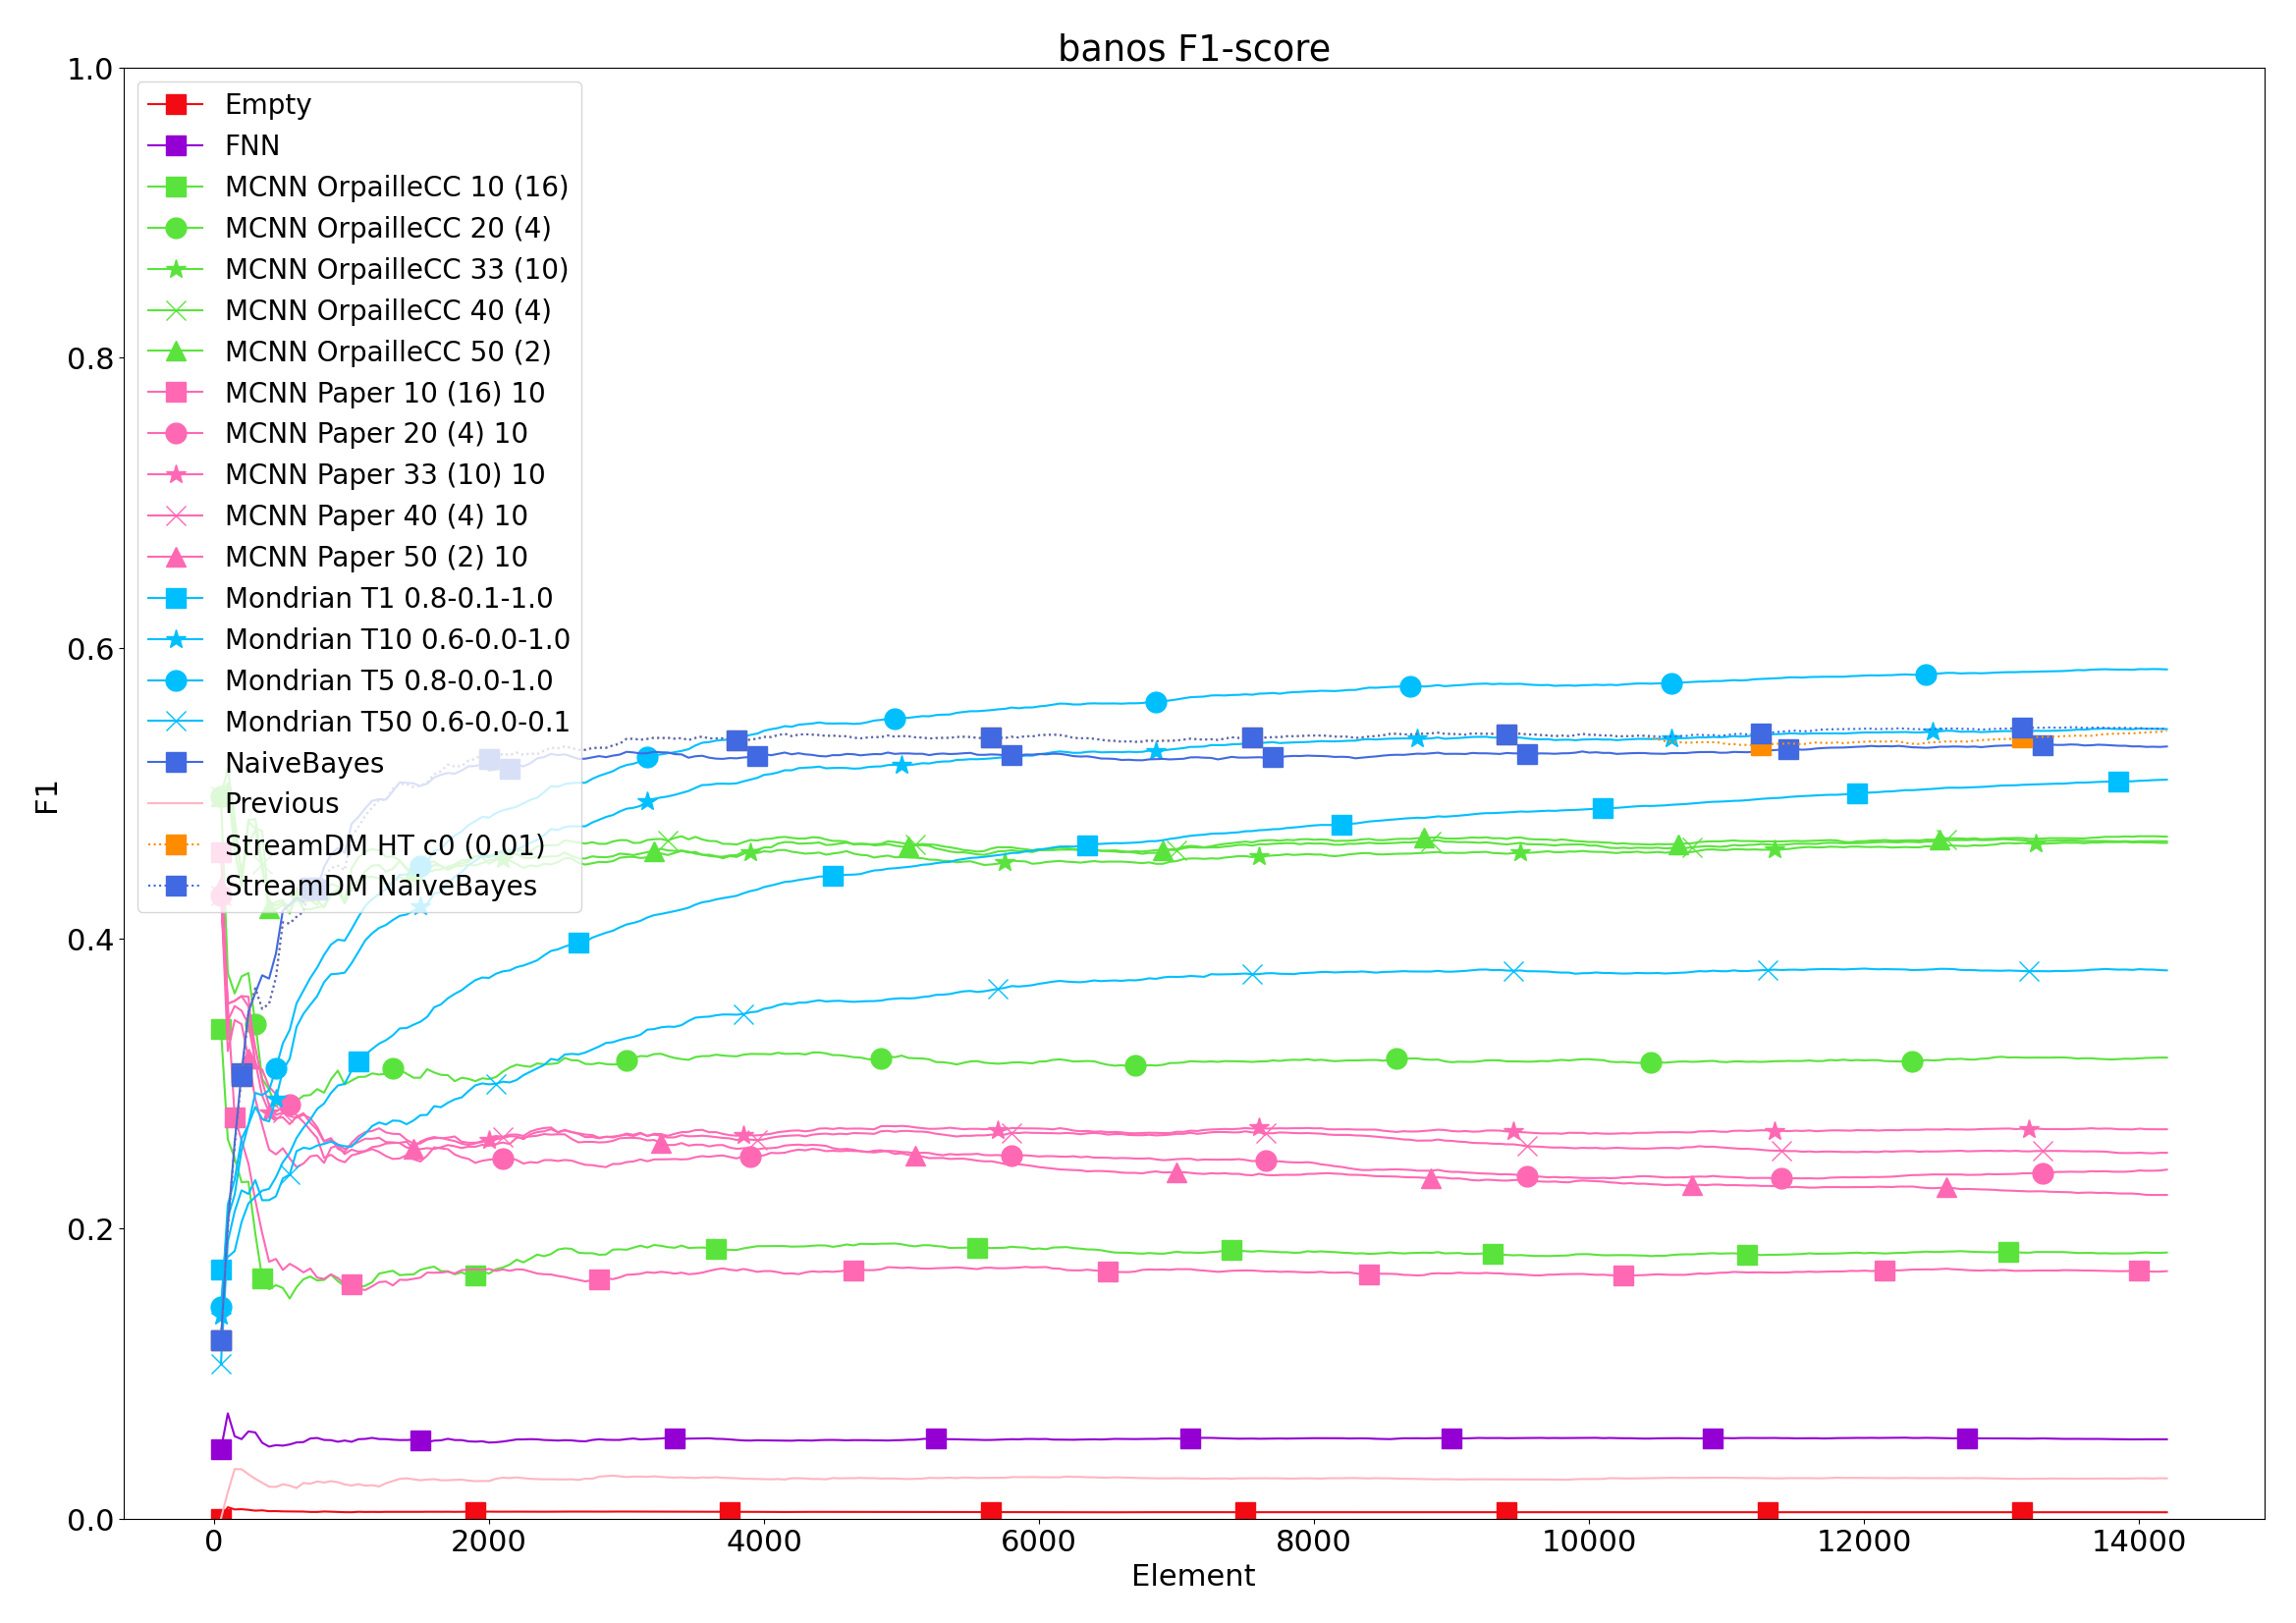
\includegraphics[width=\linewidth]{figures/results/banos_f1.png}
	\caption{F1-score on the Banos dataset.}
\end{figure}
\begin{figure}[H]
	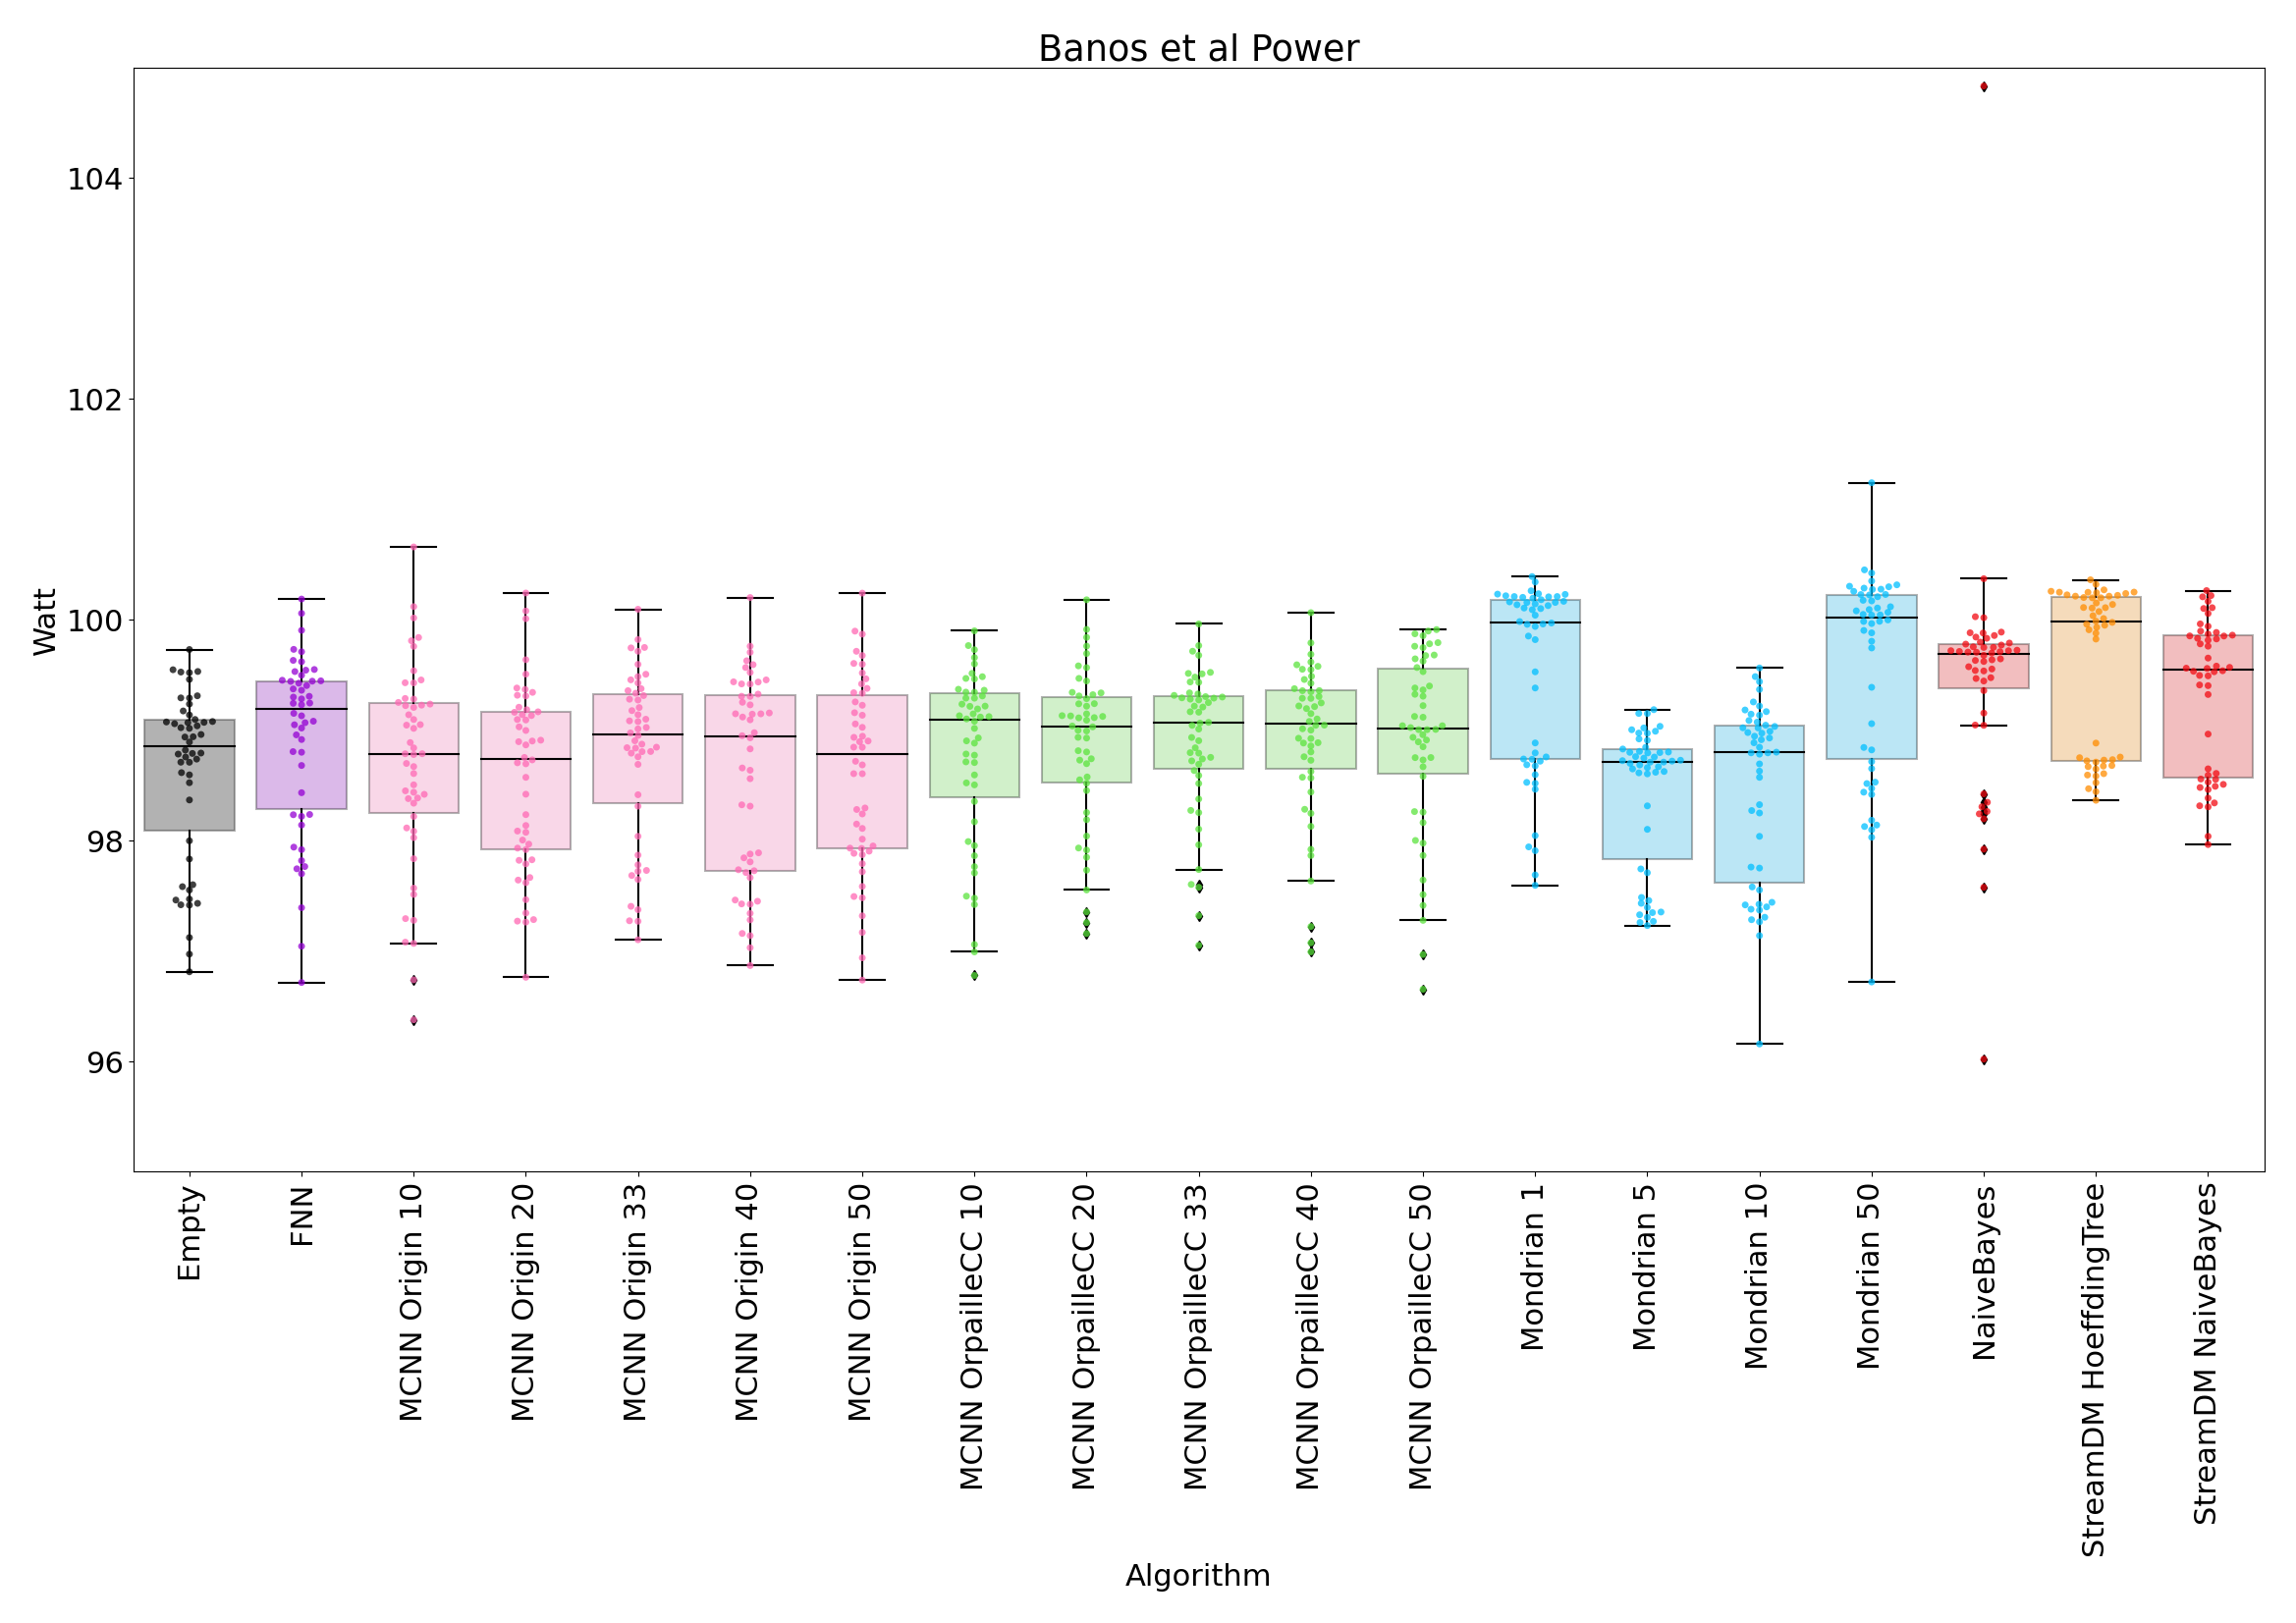
\includegraphics[width=\linewidth]{figures/results/banos_watt.png}
	\caption{Power needed for each algorithm on the Banos dataset.}
\end{figure}
\begin{figure}[H]
	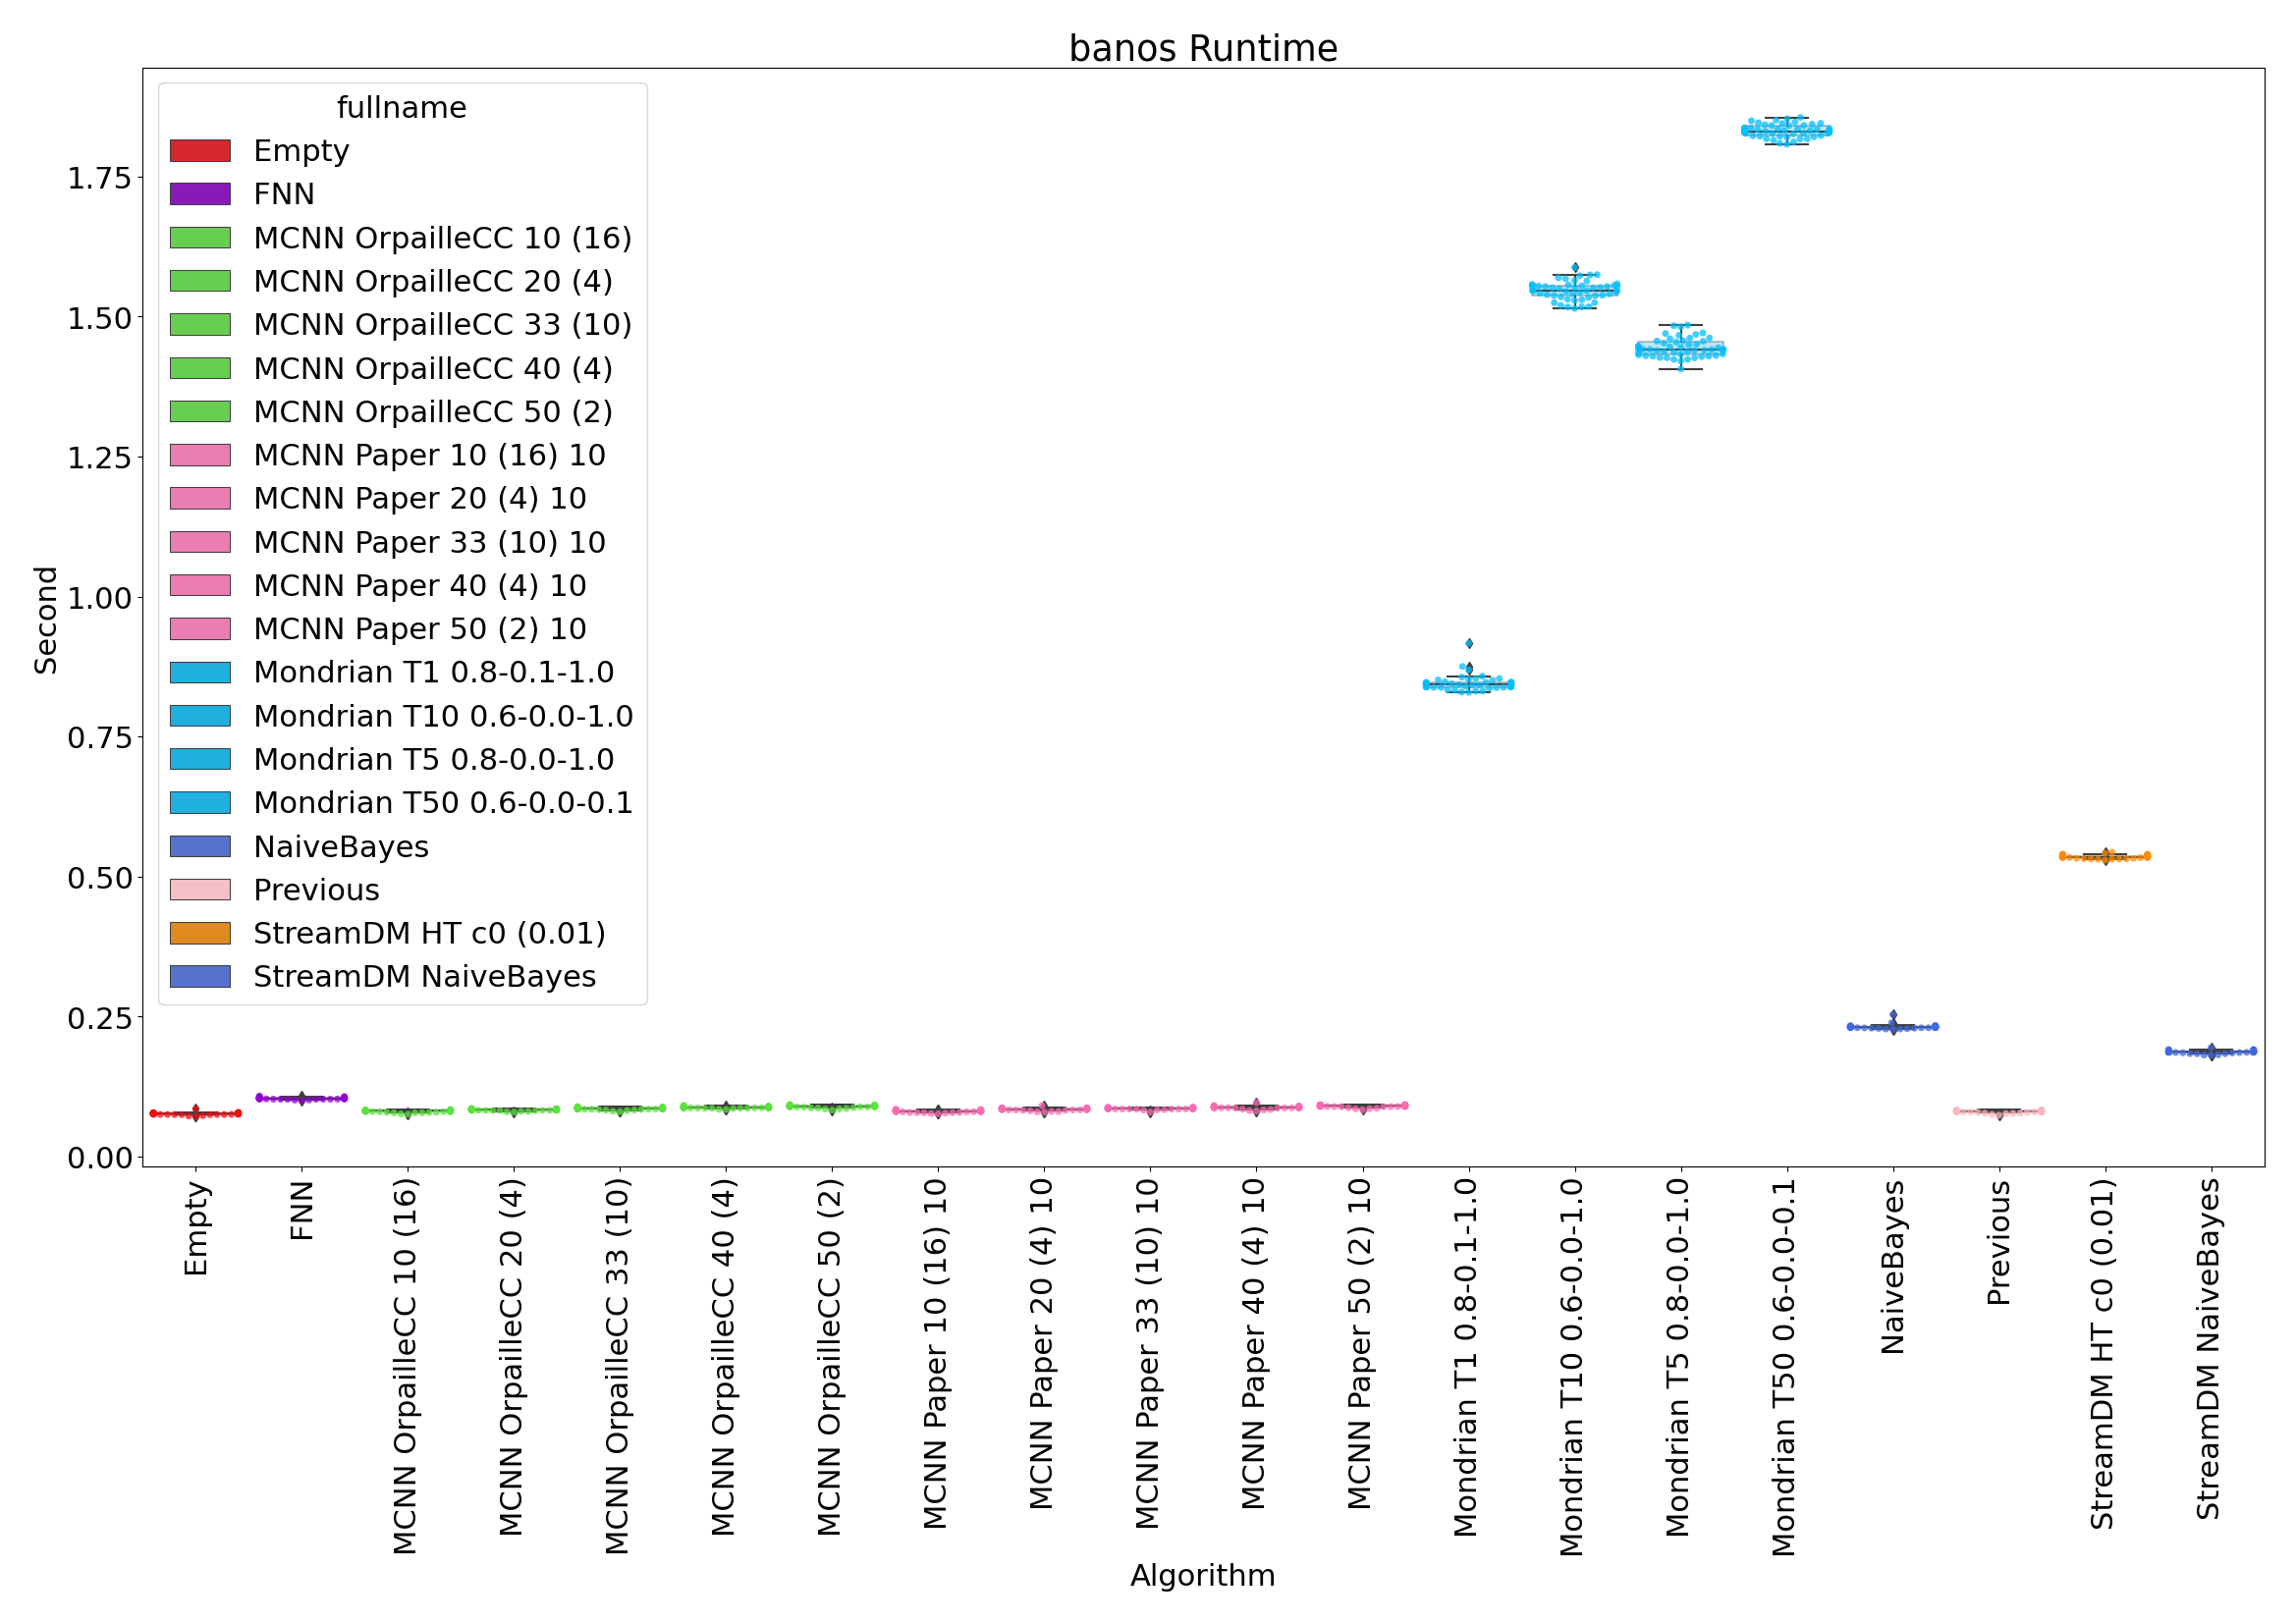
\includegraphics[width=\linewidth]{figures/results/banos_runtime.png}
	\caption{Runtime on the Banos dataset.}
\end{figure}
\begin{figure}[H]
	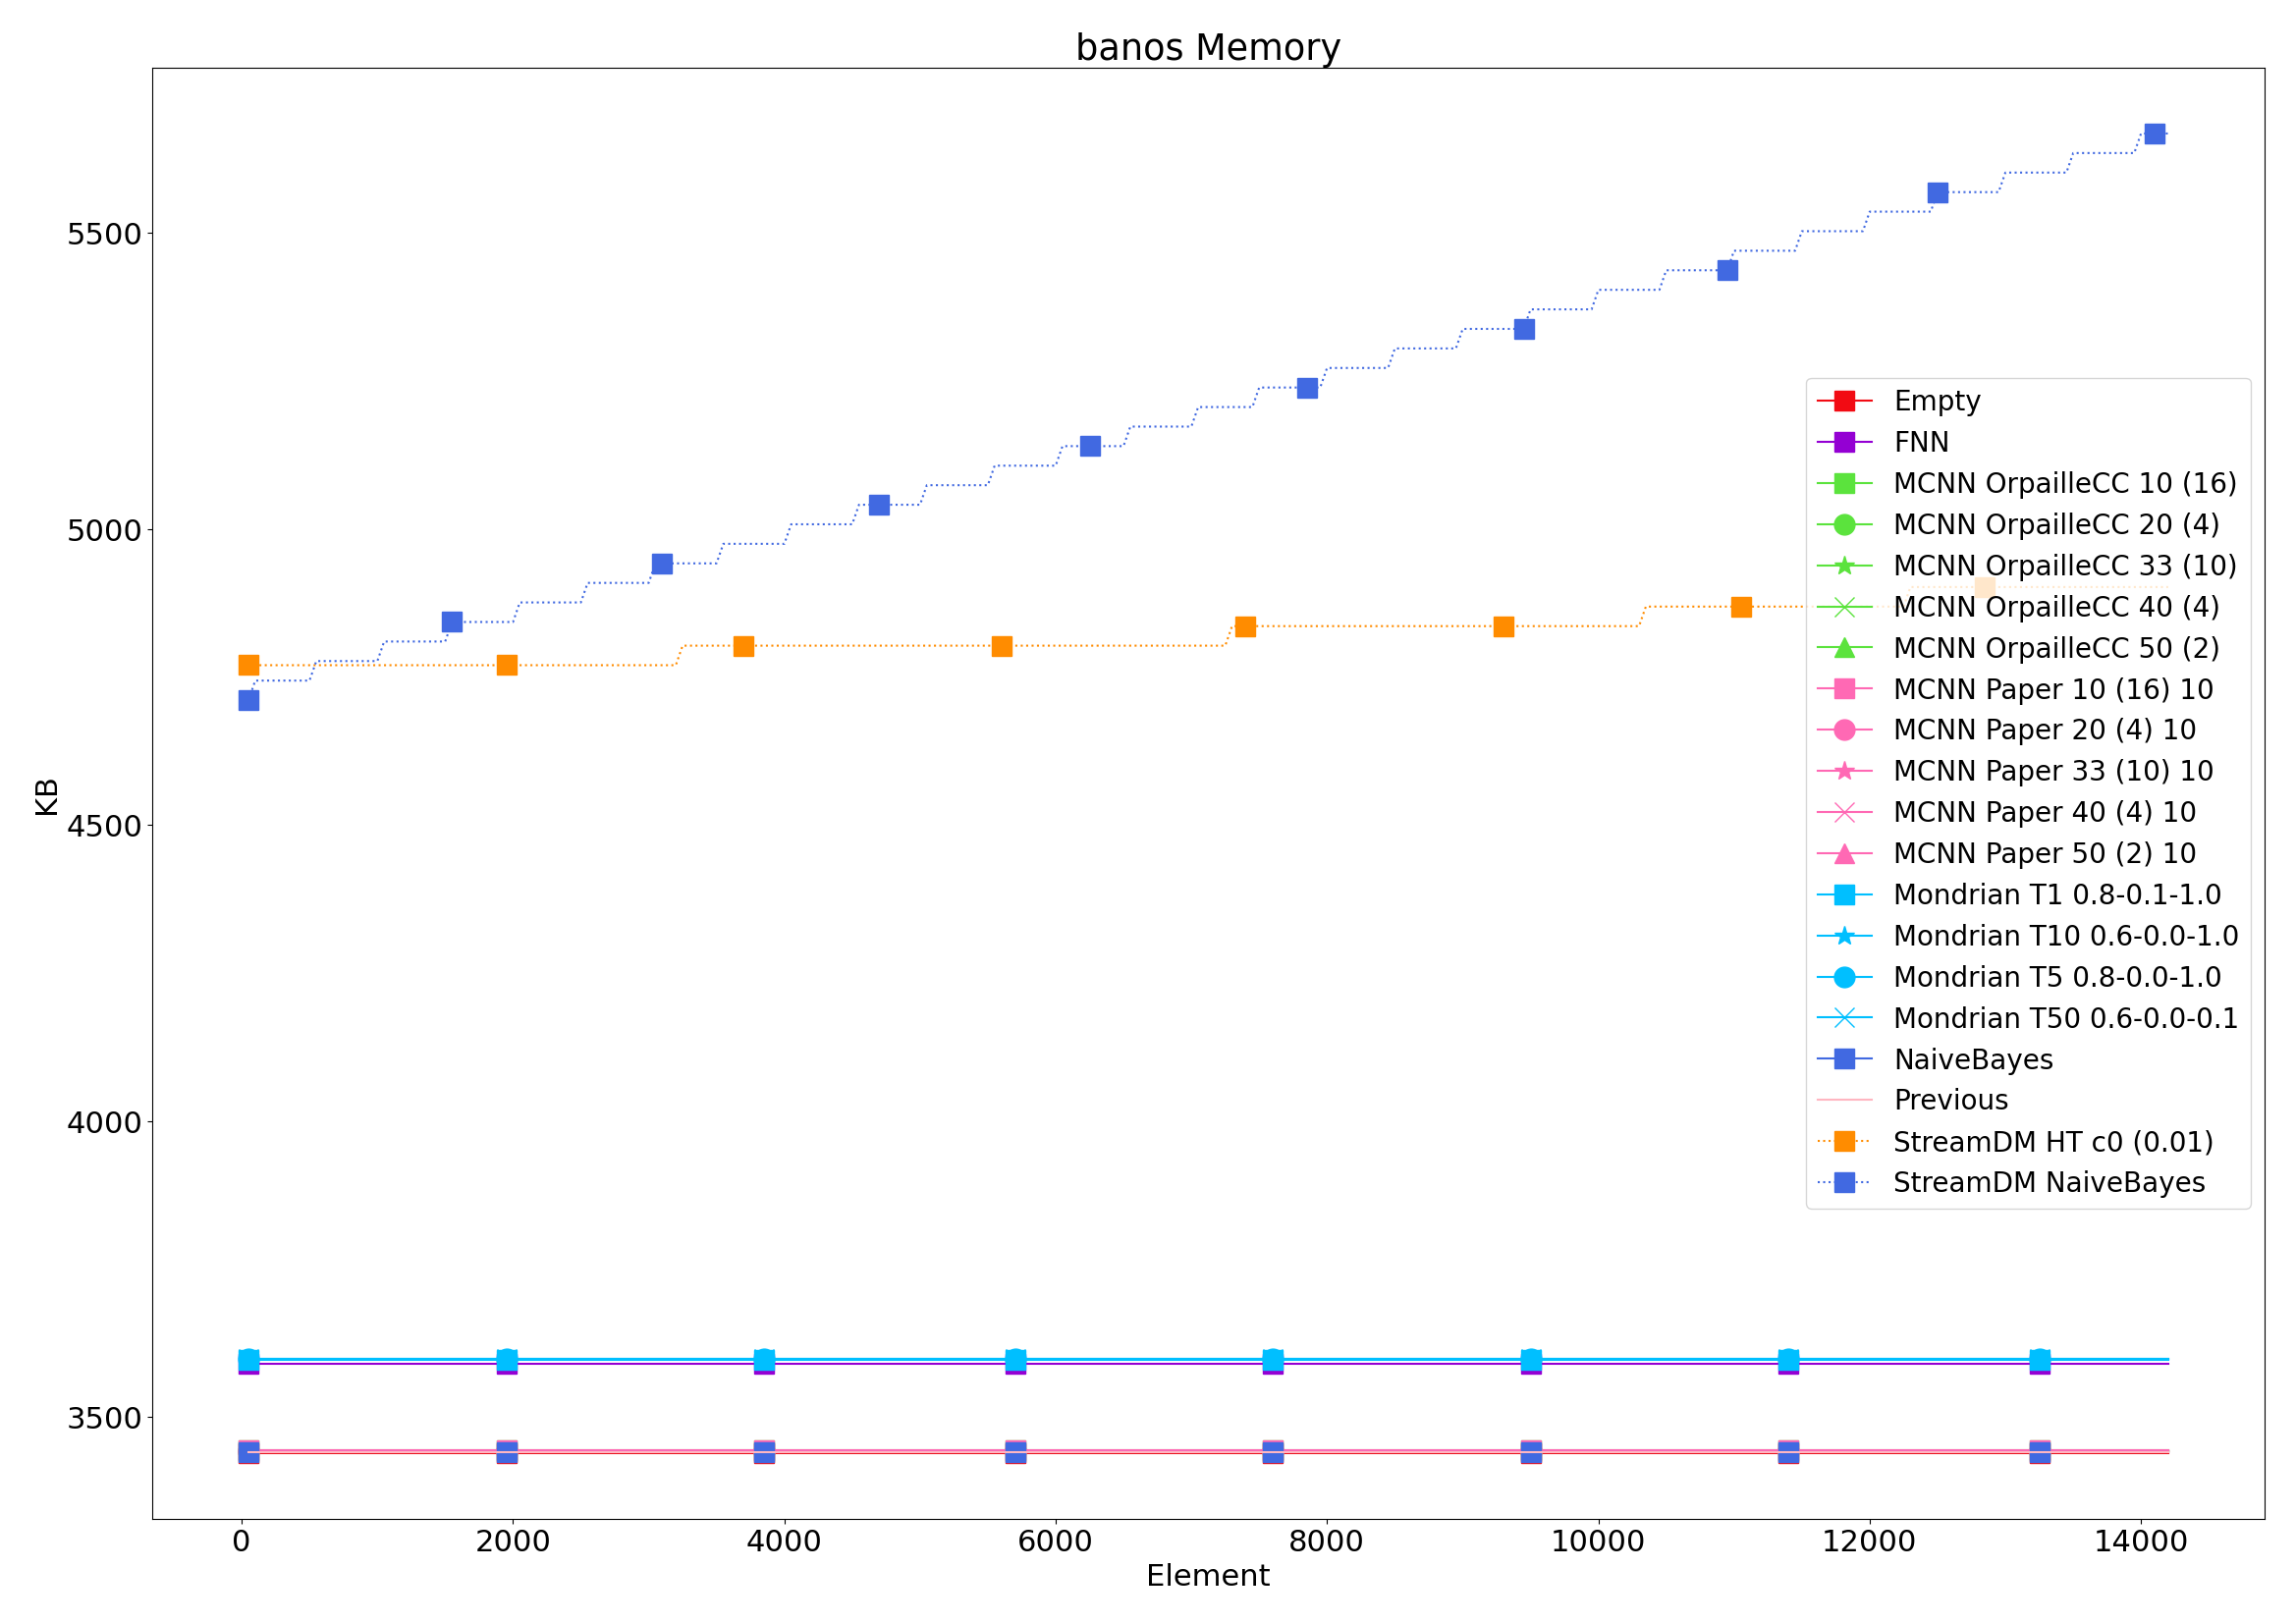
\includegraphics[width=\linewidth]{figures/results/banos_memory.png}
	\caption{Memory used by the algorithms on the Banos dataset.}
\end{figure}
\begin{figure}[H]
	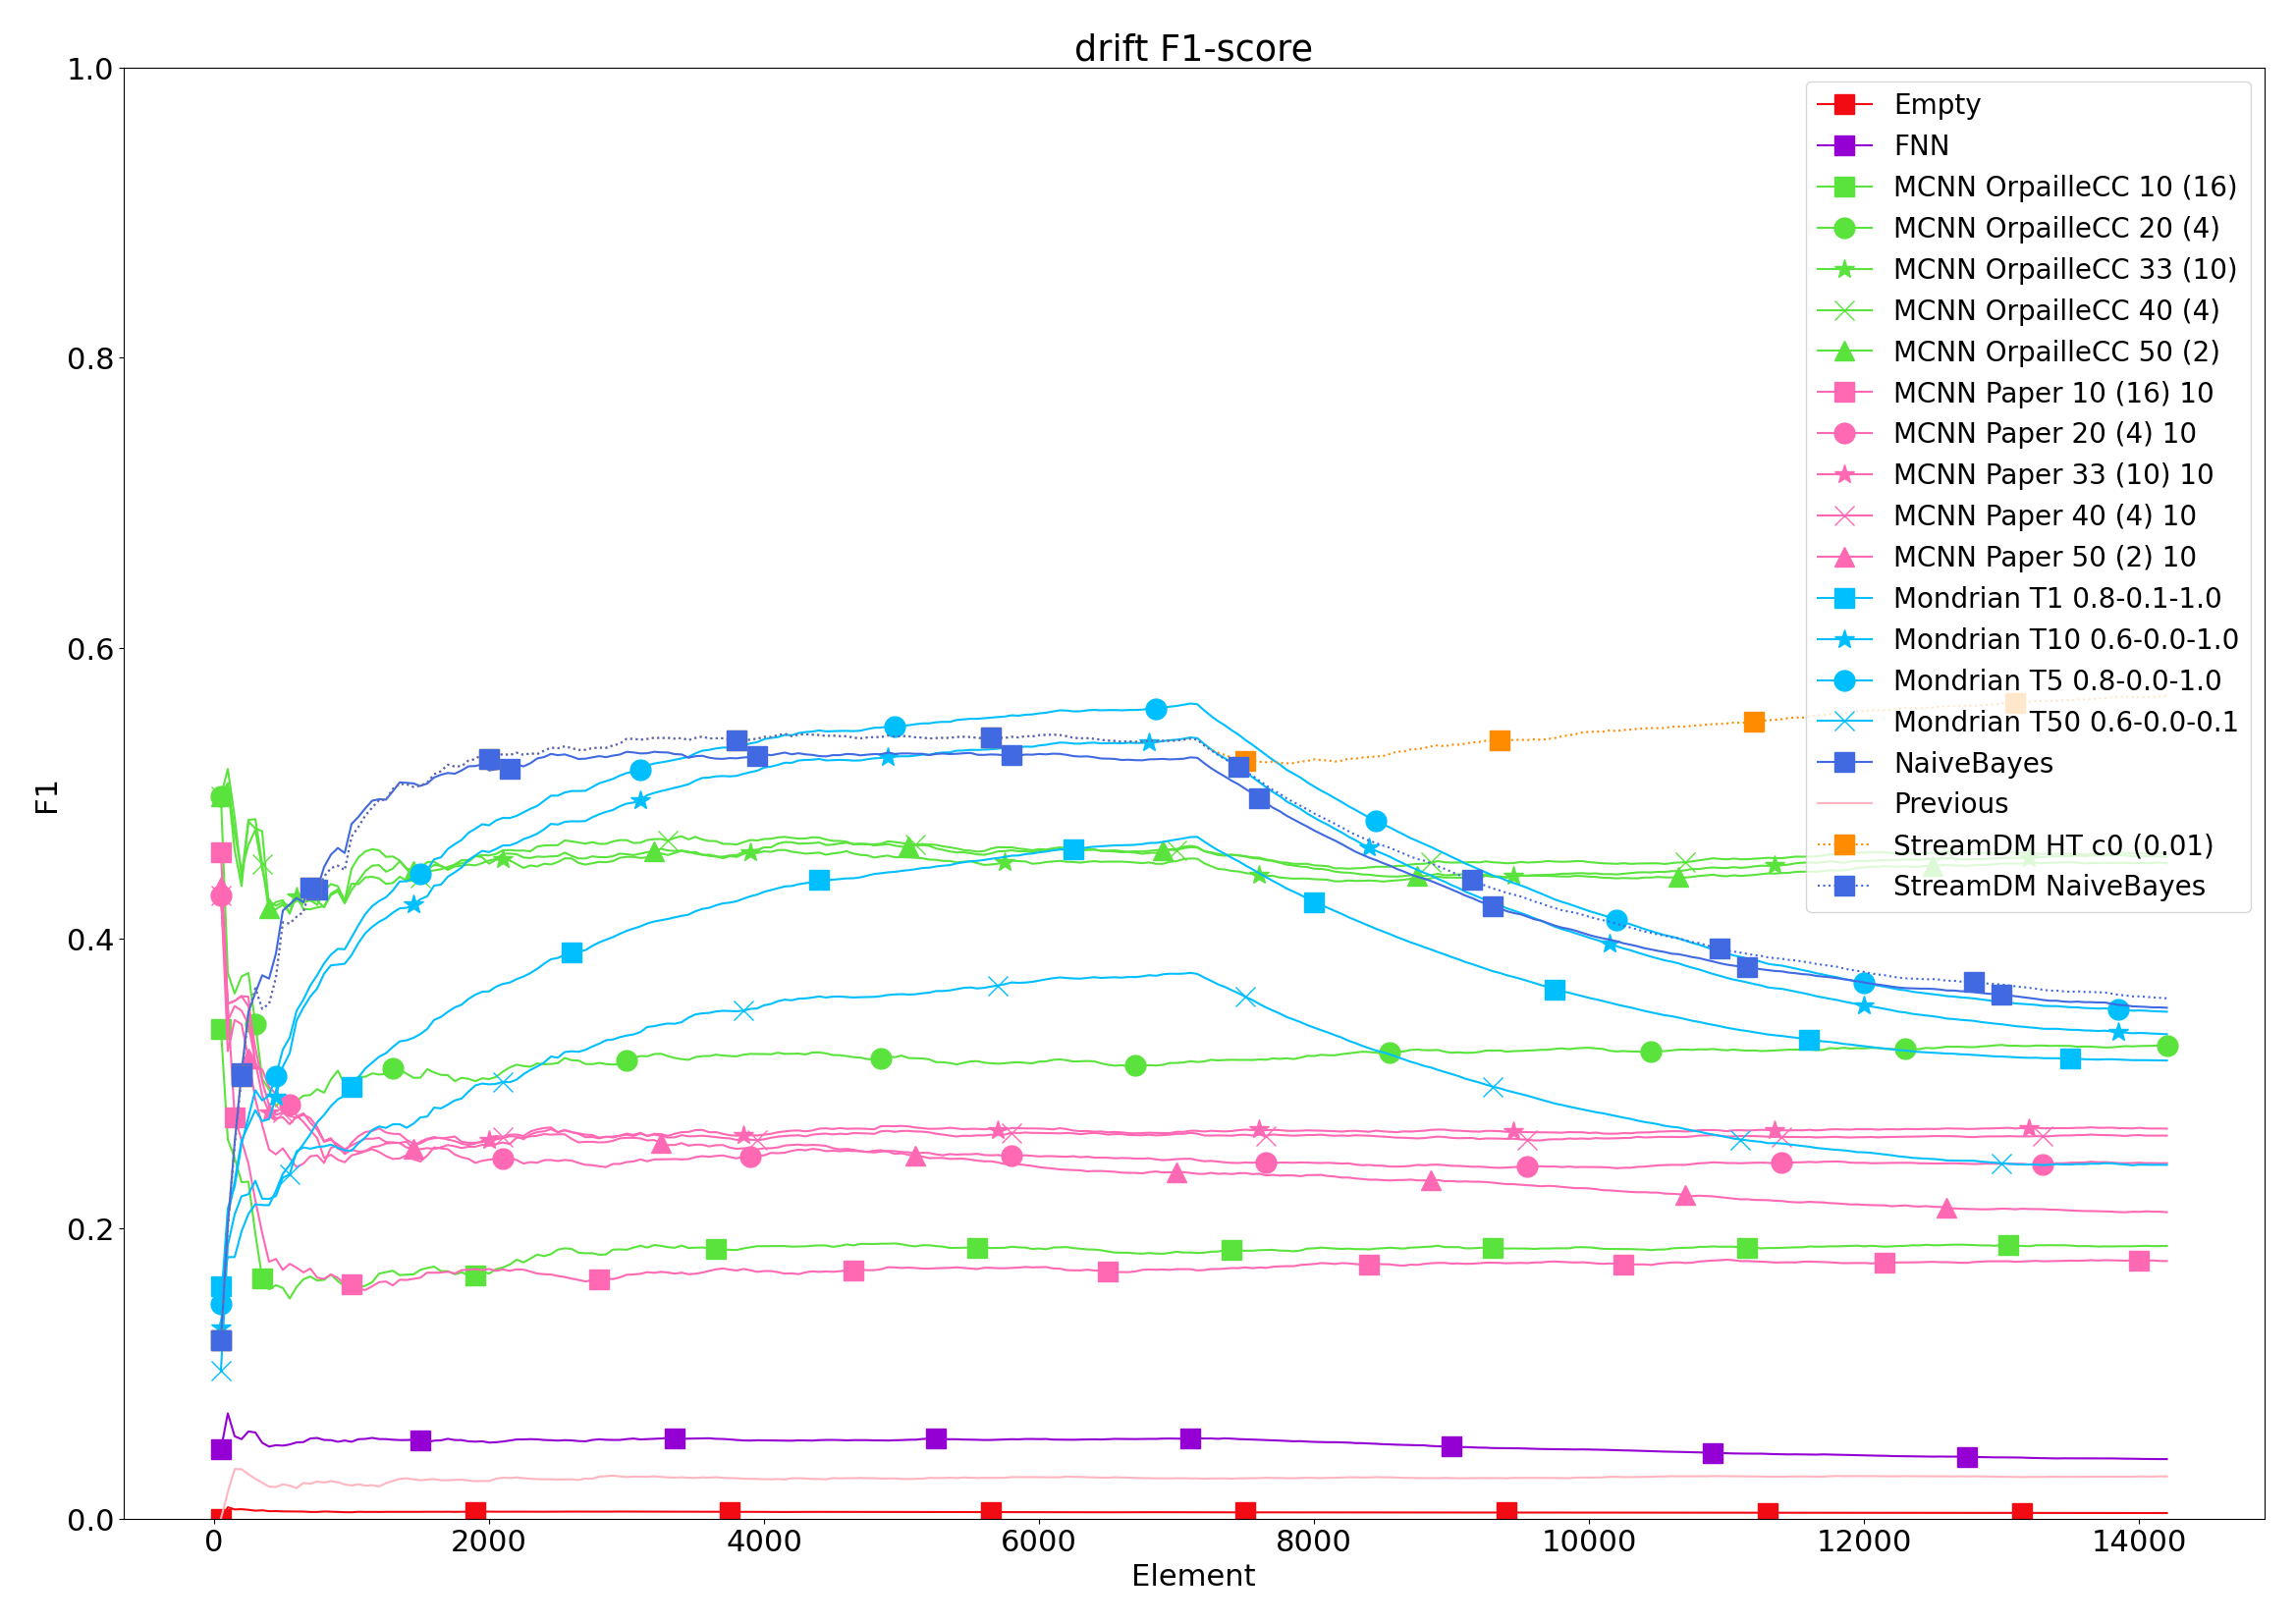
\includegraphics[width=\linewidth]{figures/results/drift_f1.png}
	\caption{Impact of an artificial drift.}
\end{figure}

\subsection{Recofit results}
Figure show the accuracy on the Recofit dataset.

\begin{figure}[H]
	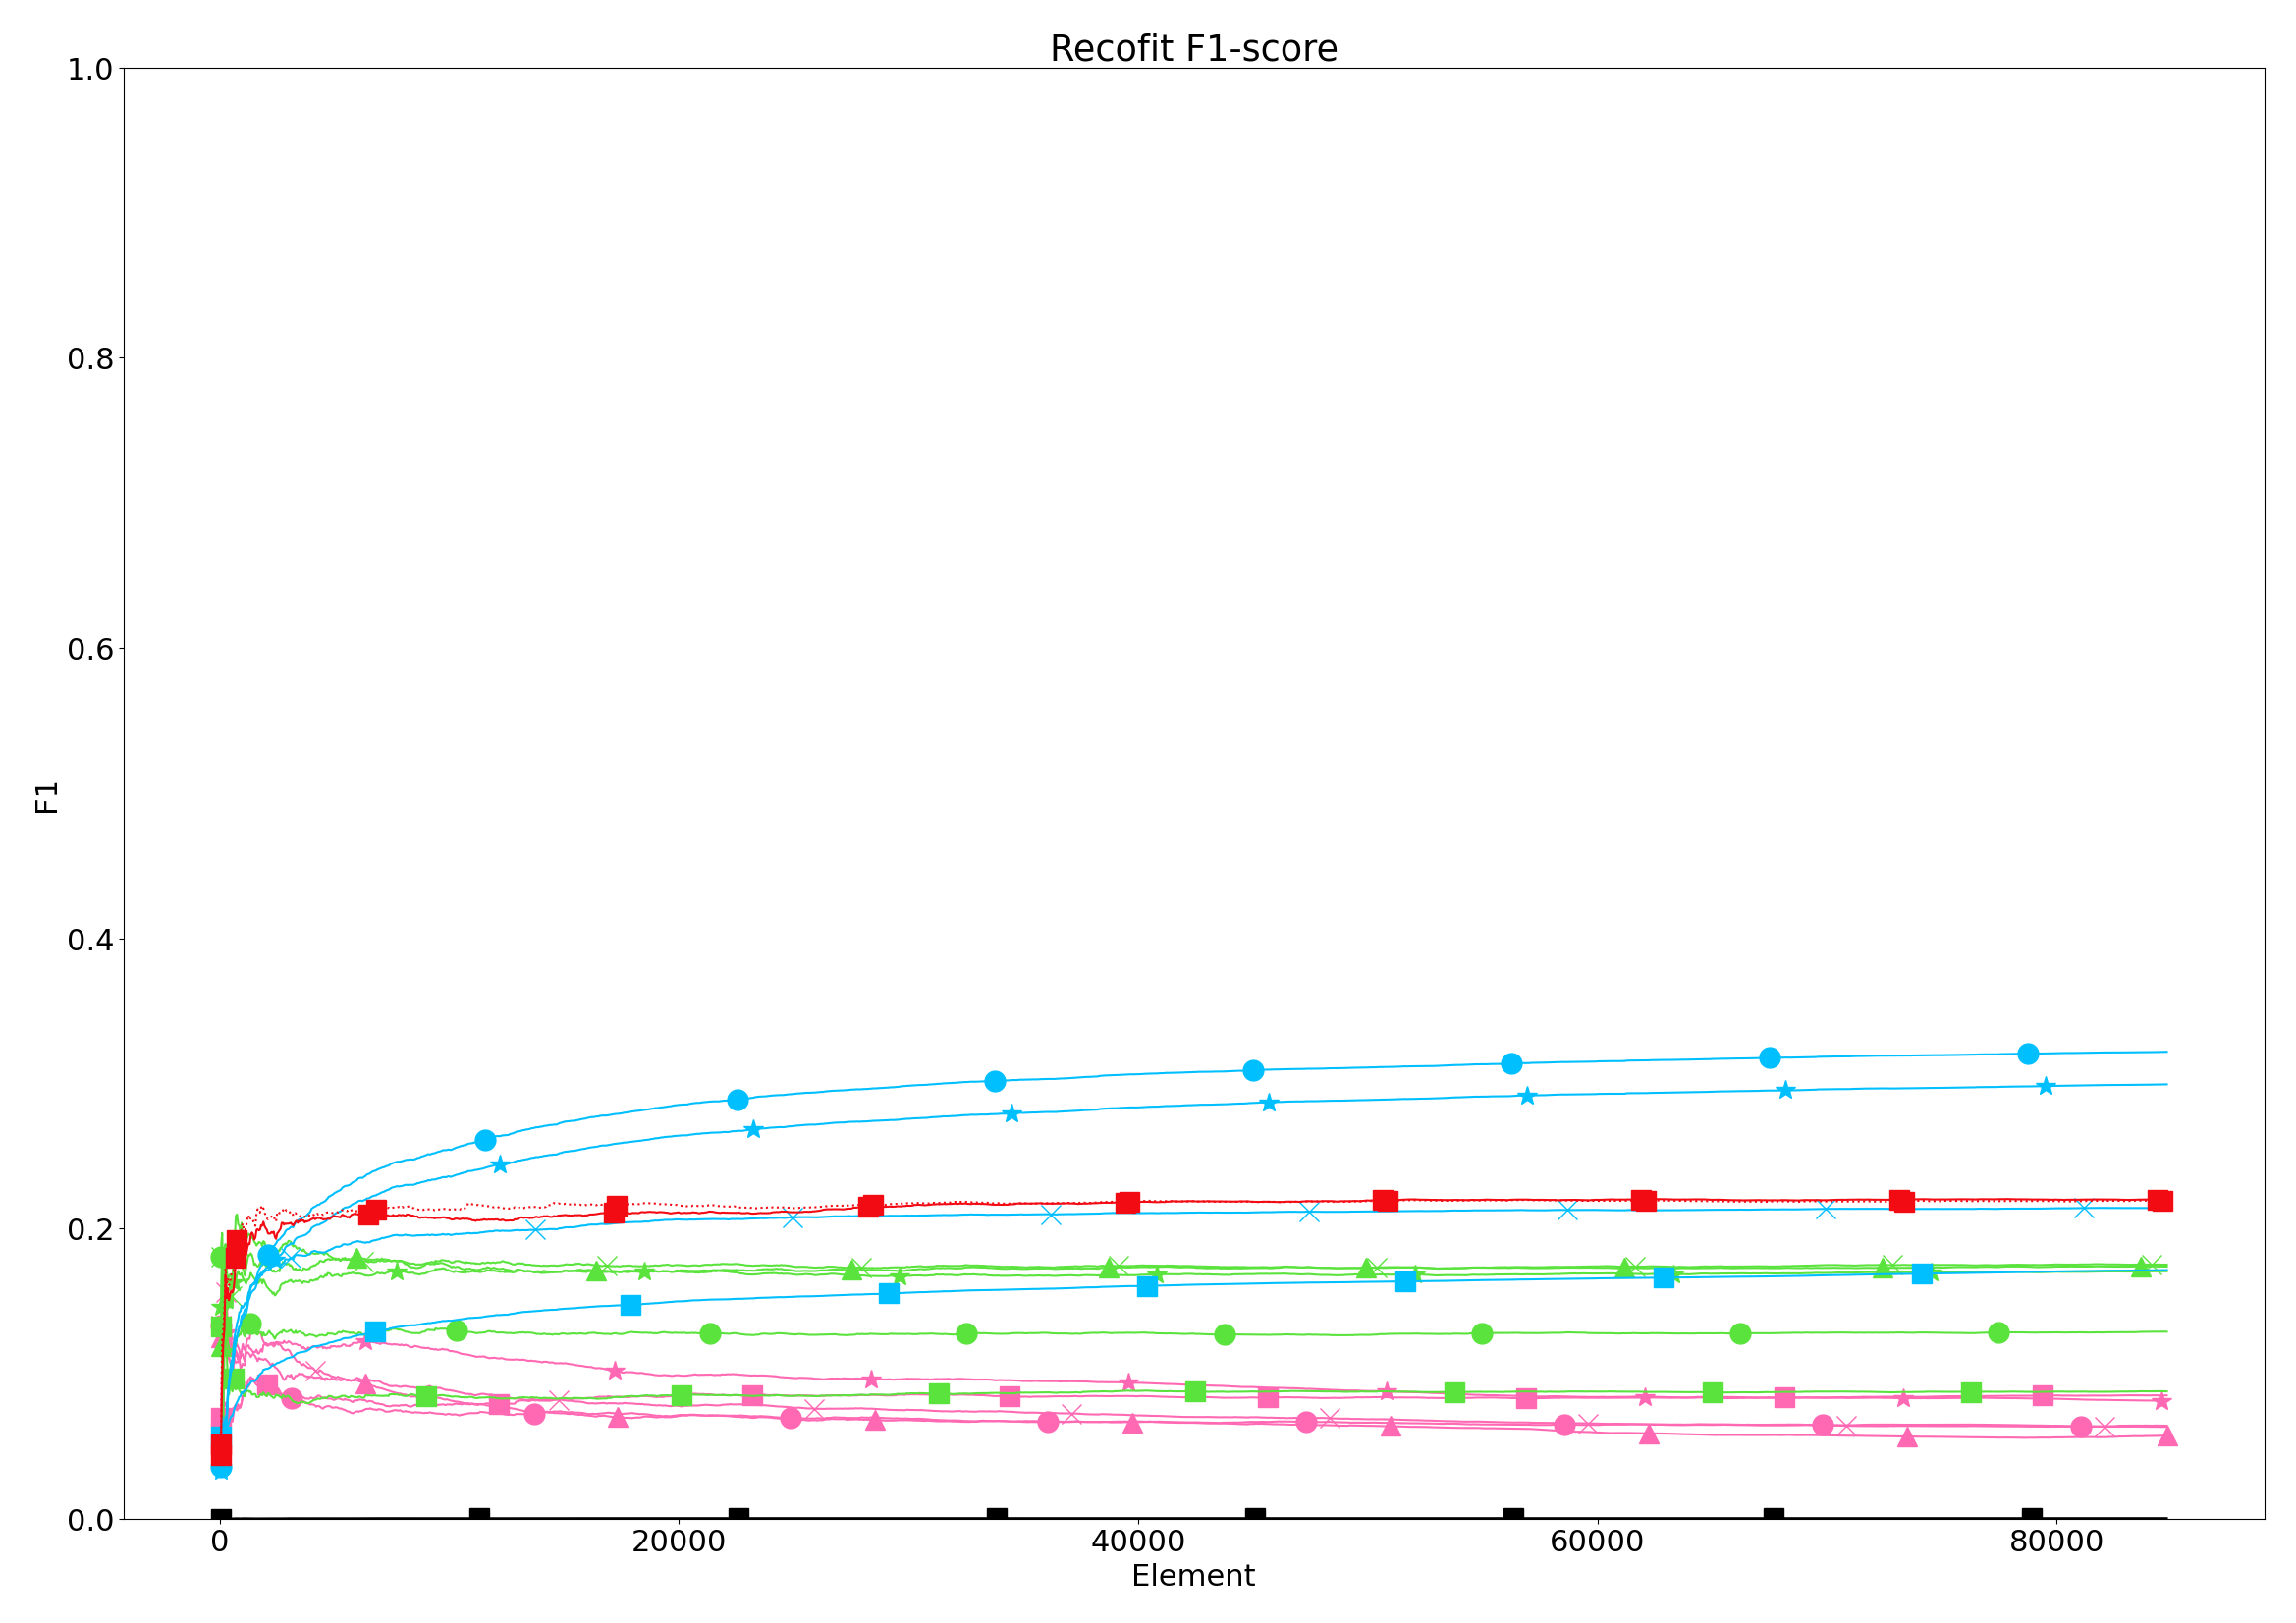
\includegraphics[width=\linewidth]{figures/results/recofit_f1.png}
	\caption{F1-score on the Recofit dataset.}
\end{figure}
\begin{figure}[H]
	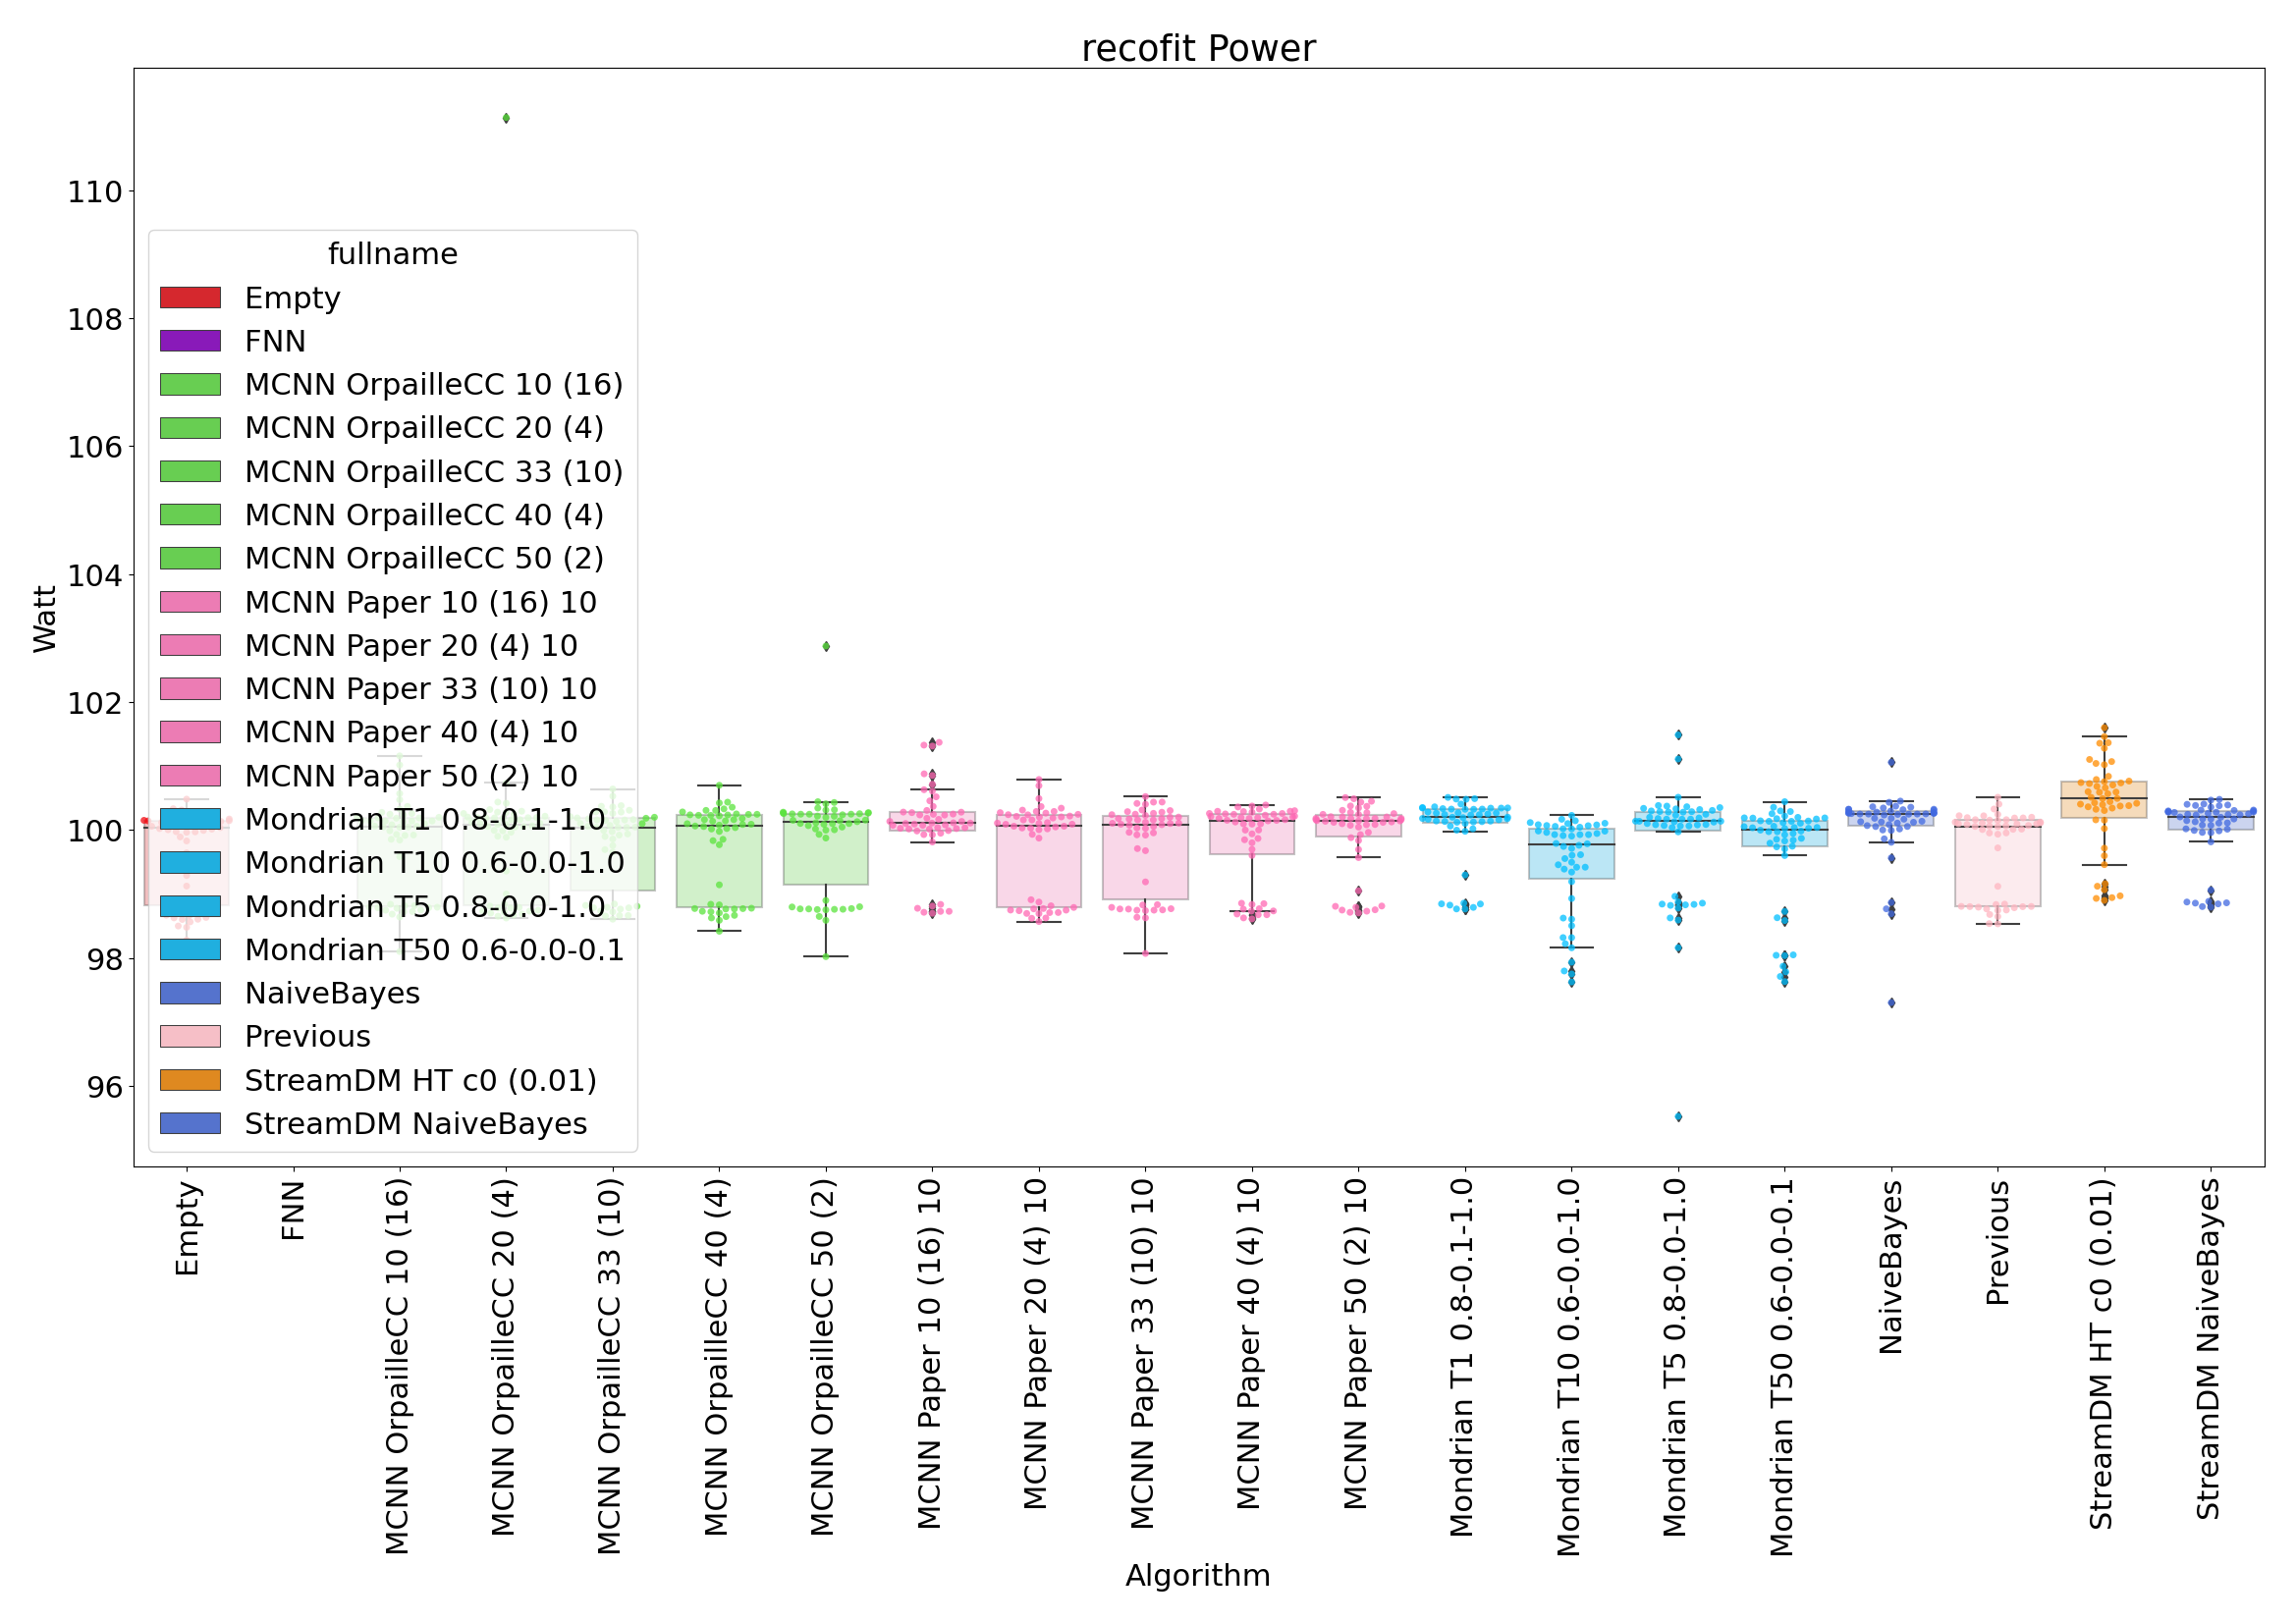
\includegraphics[width=\linewidth]{figures/results/recofit_watt.png}
	\caption{Power needed for each algorithm on the Recofit dataset.}
\end{figure}
\begin{figure}[H]
	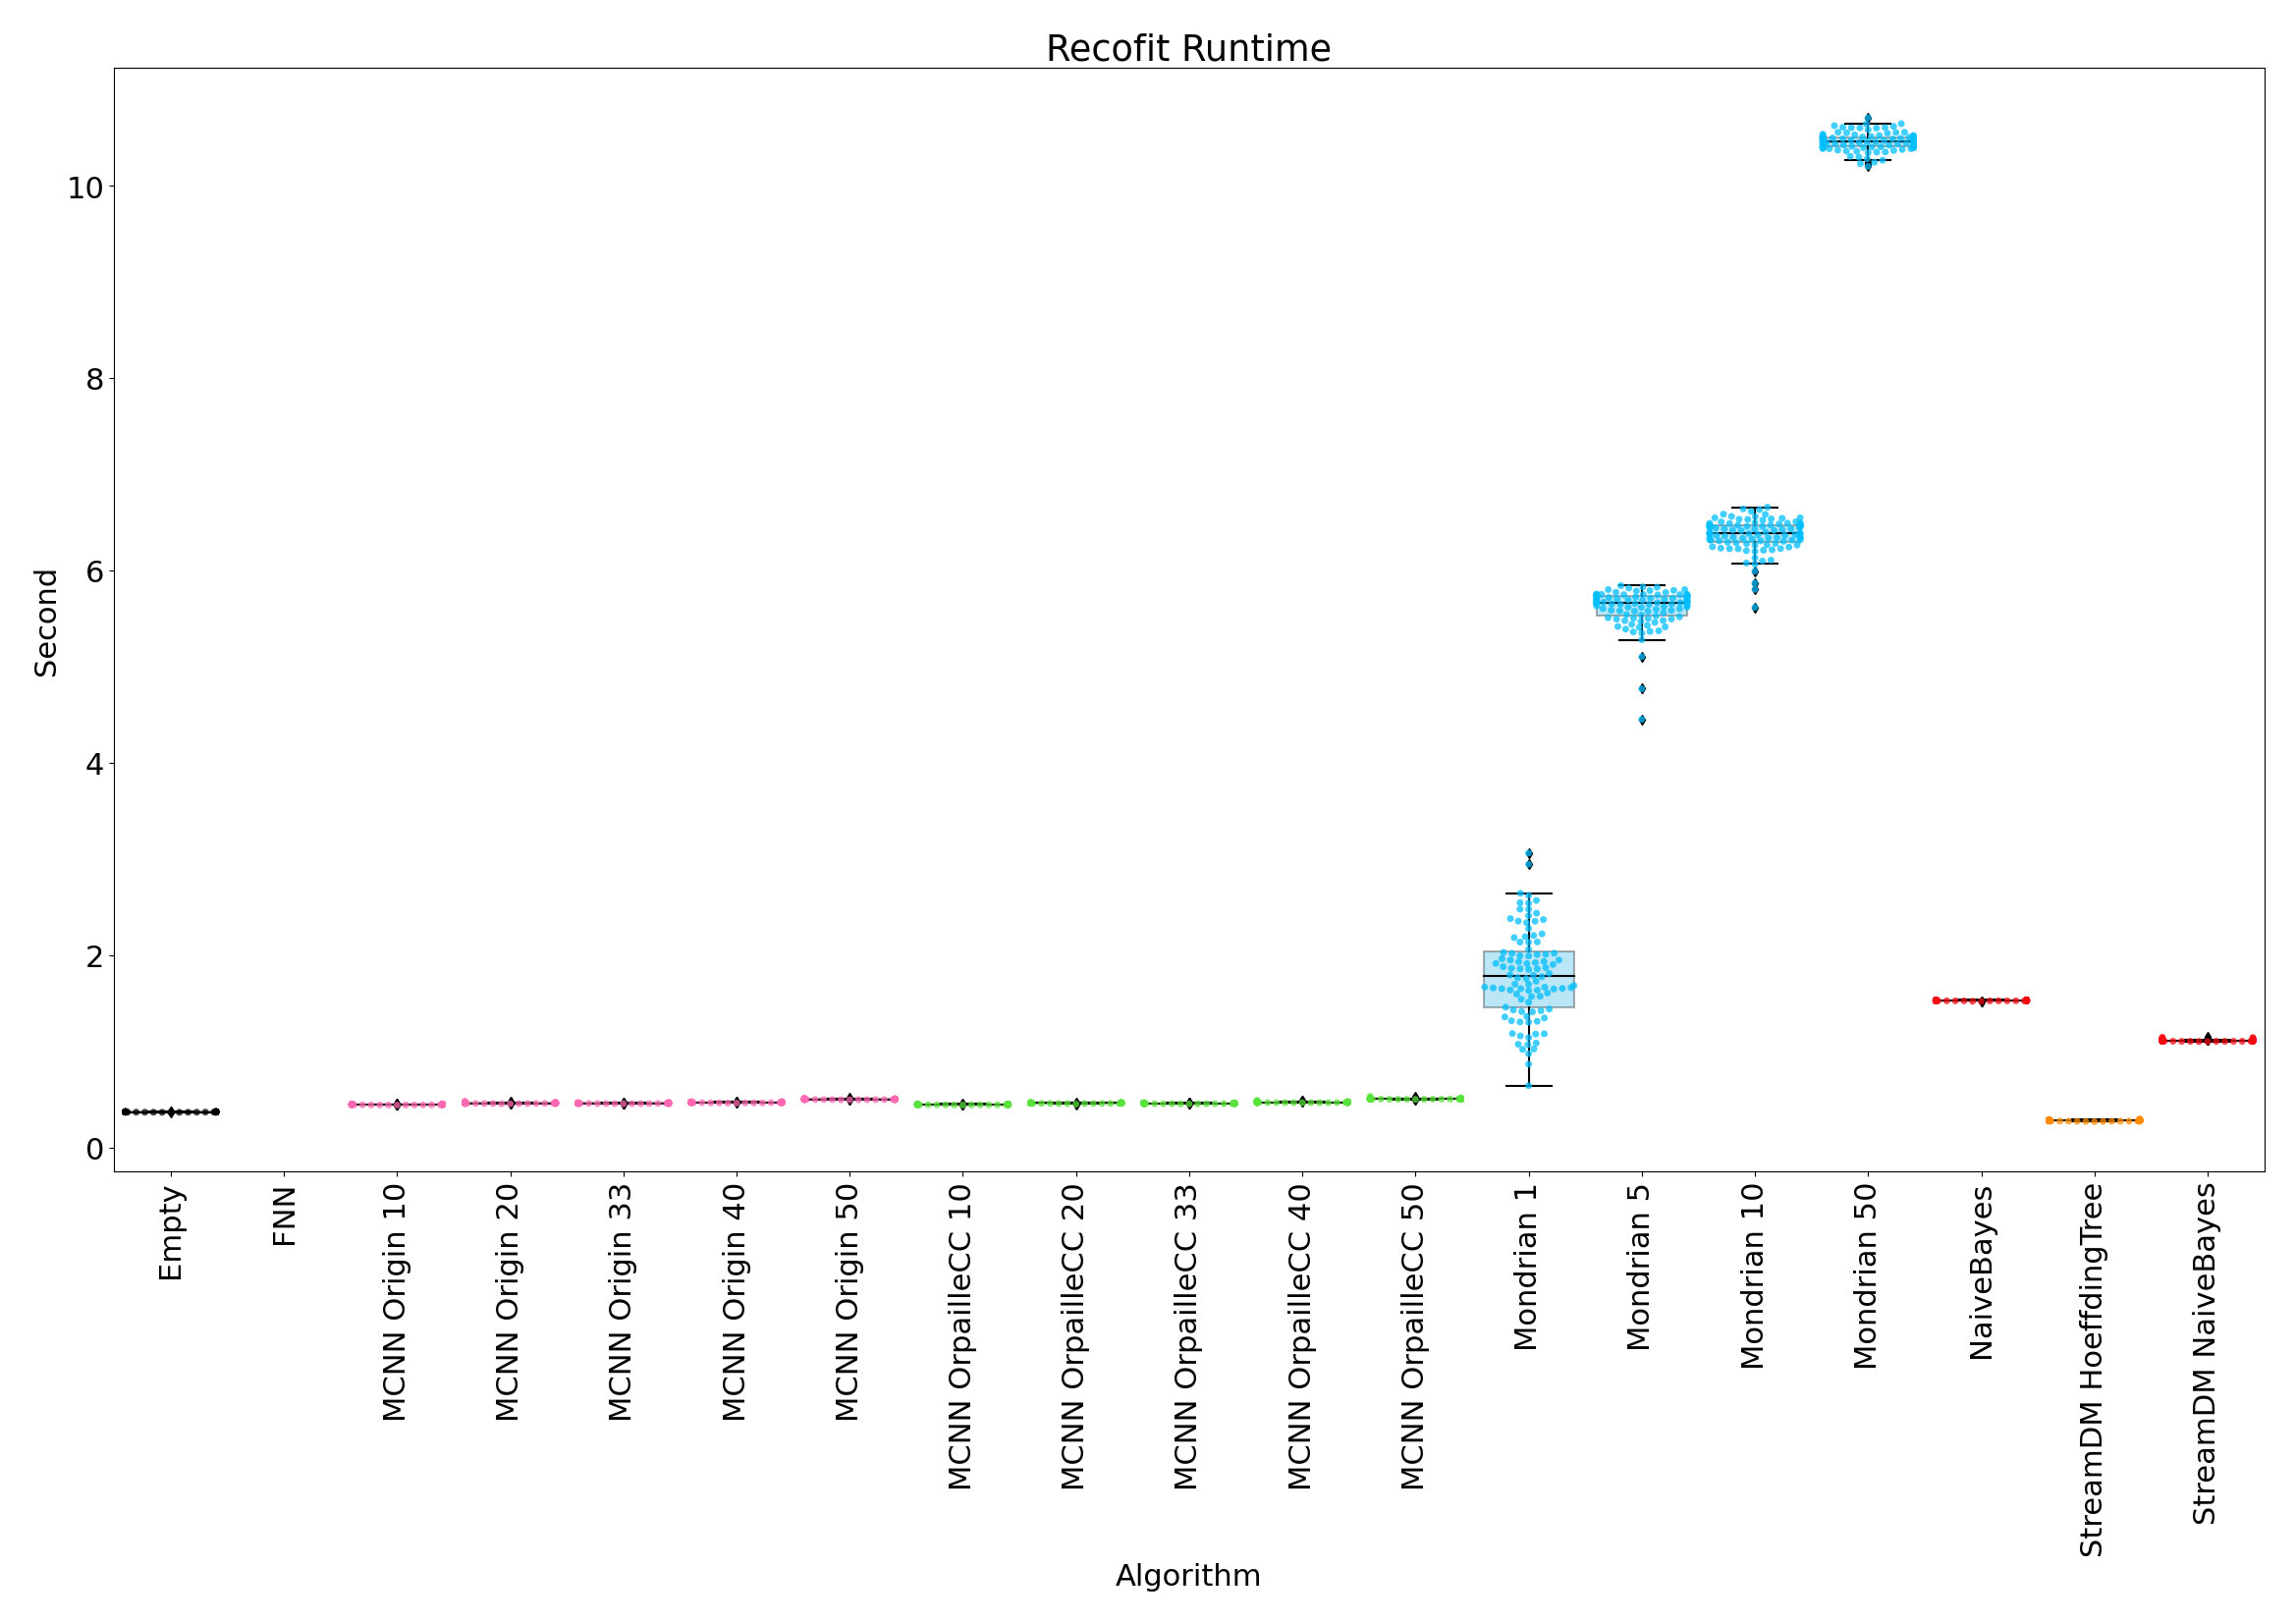
\includegraphics[width=\linewidth]{figures/results/recofit_runtime.png}
	\caption{Runtime on the Recofit dataset.}
\end{figure}

\subsection{Synthetic datasets results}
Figure show the accuracy on the Recofit dataset.

\begin{figure}[H]
	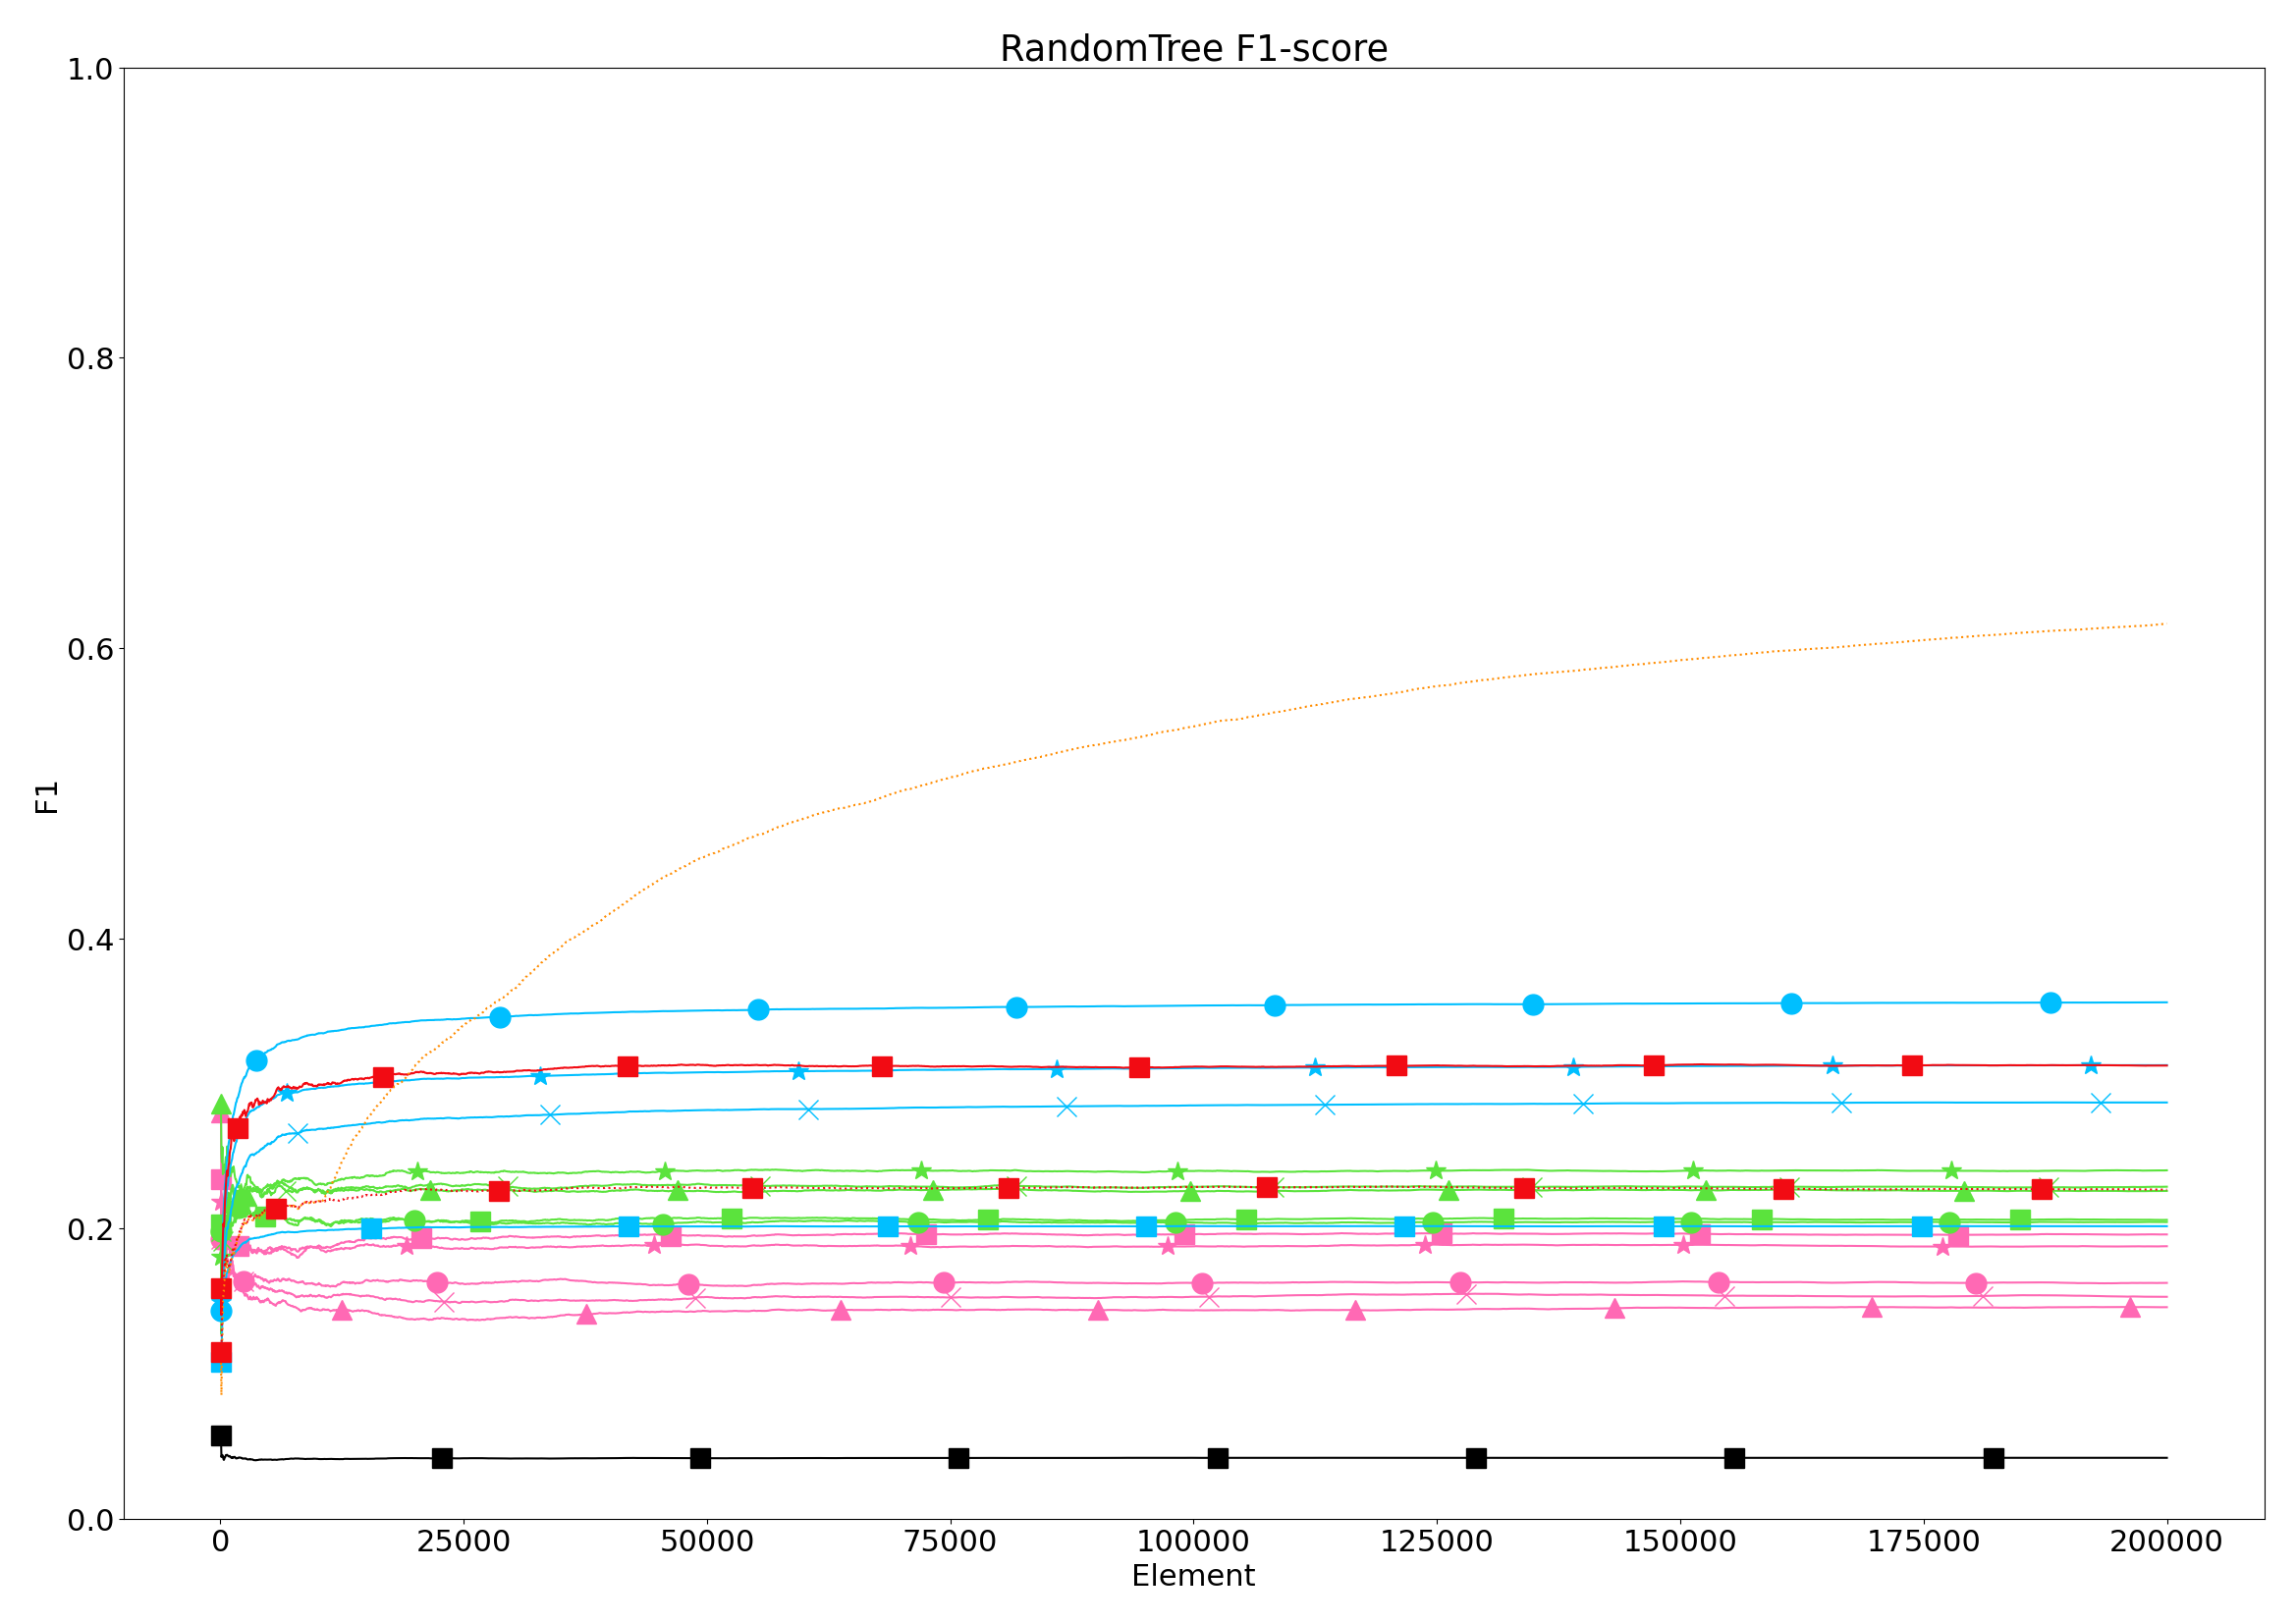
\includegraphics[width=\linewidth]{figures/results/dataset_3_f1.png}
	\caption{F1-score on the third synthetic dataset.}
\end{figure}
\begin{figure}[H]
	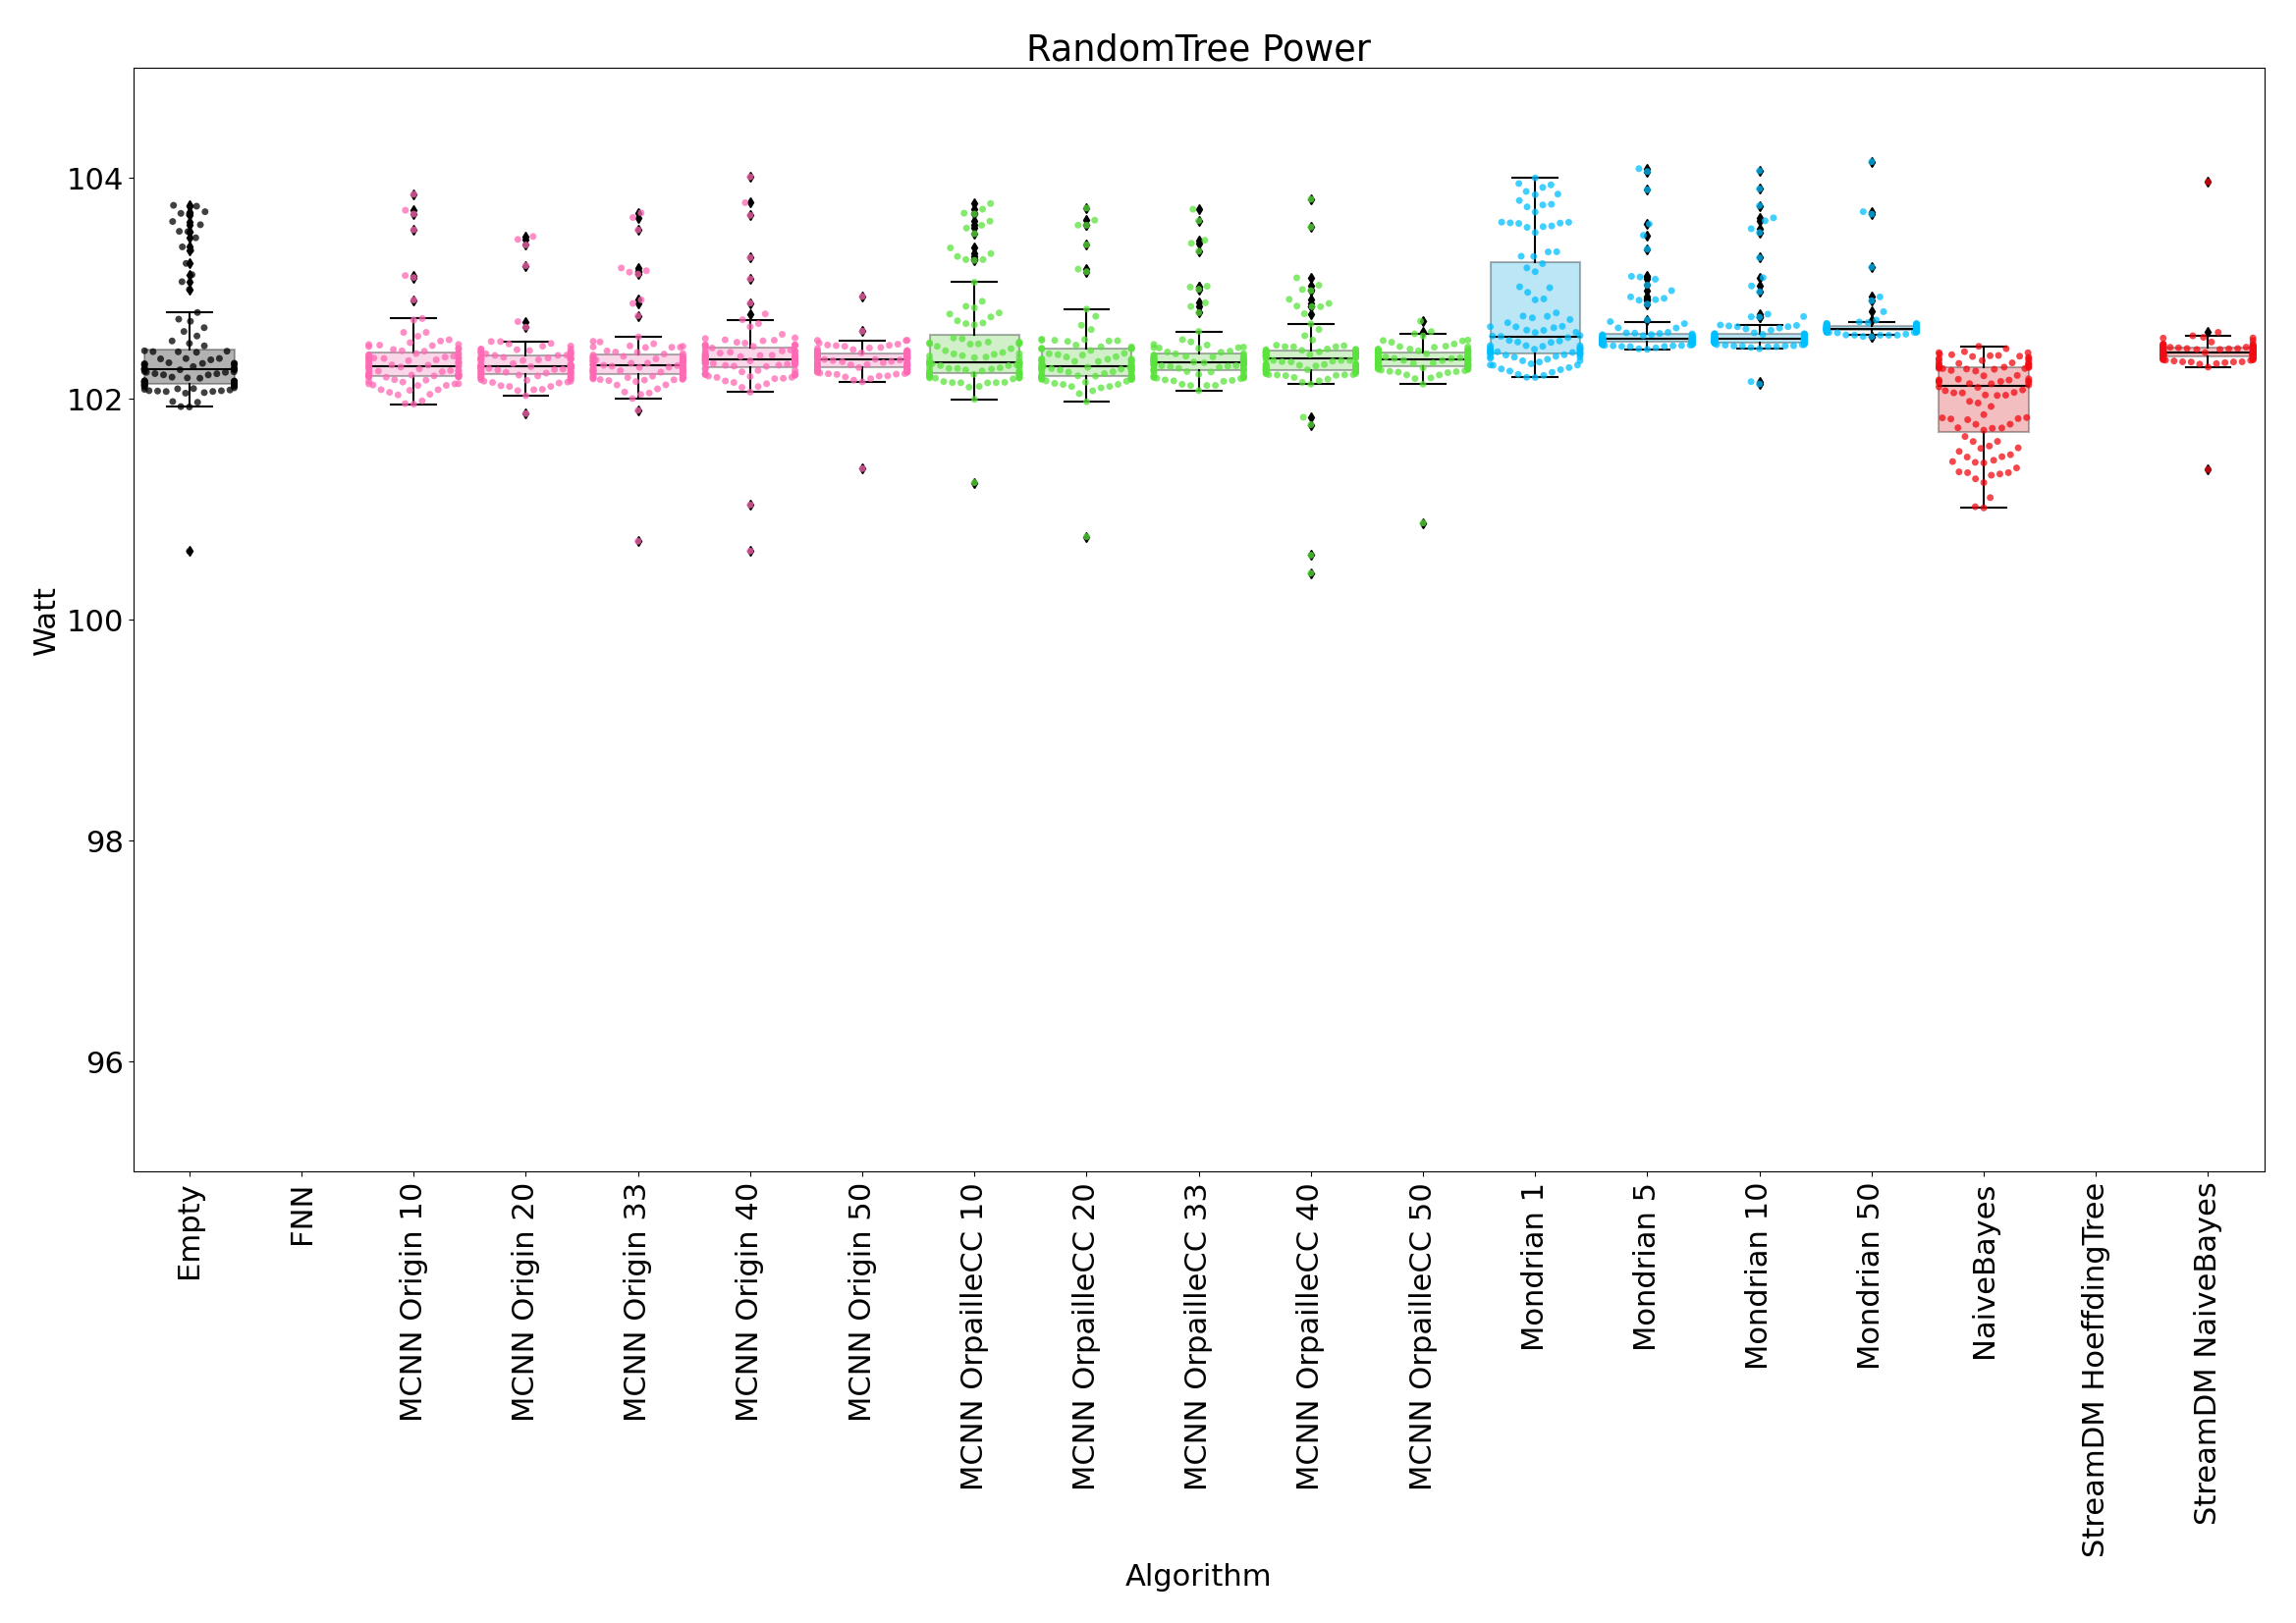
\includegraphics[width=\linewidth]{figures/results/dataset_3_watt.png}
	\caption{Power needed for each algorithm on the third synthetic dataset.}
\end{figure}
\subsection{Micro-Cluster Nearest Neighbor tuning}
Figure~\ref{fig:mcnn-tuning-error} show the impact of the error threshold on different number of cluster.
\begin{figure}[H]
     \begin{subfigure}[b]{0.49\textwidth}
         \centering
		 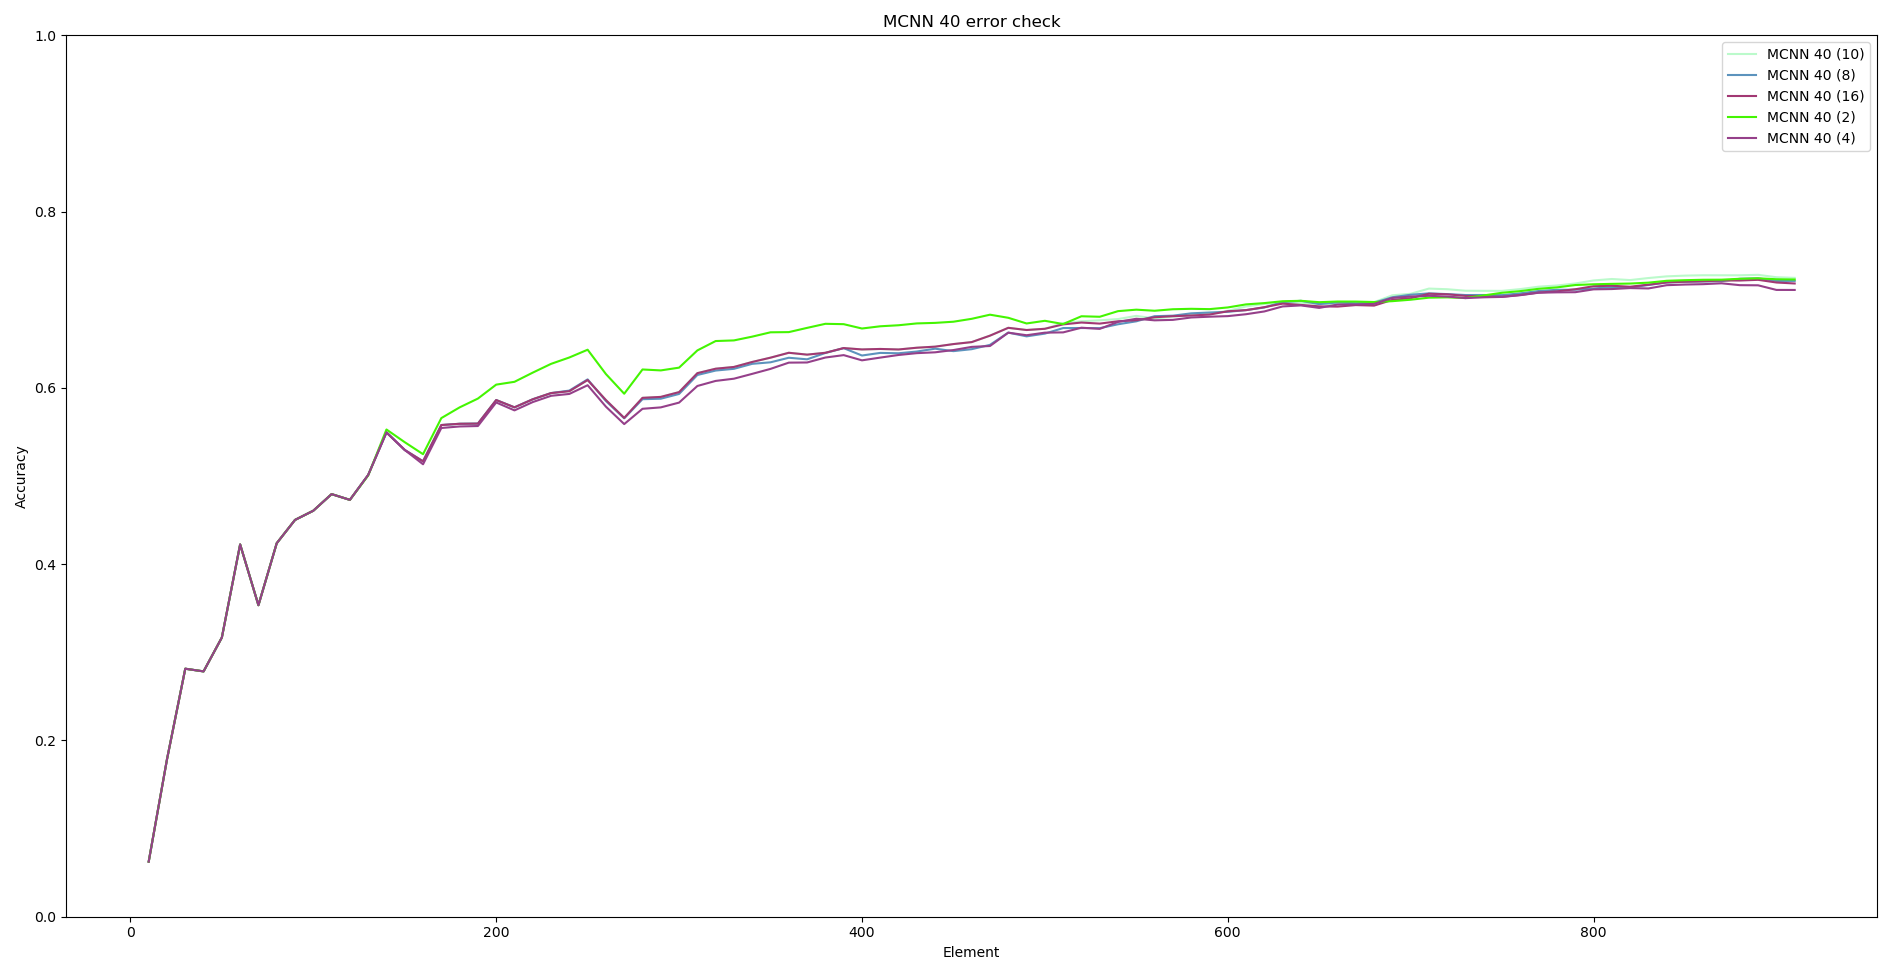
\includegraphics[width=\linewidth]{figures/Banos_S1_shuf_MCNN_40_error_check.png}
         \caption{40 clusters}
     \end{subfigure}
     \begin{subfigure}[b]{0.49\textwidth}
         \centering
		 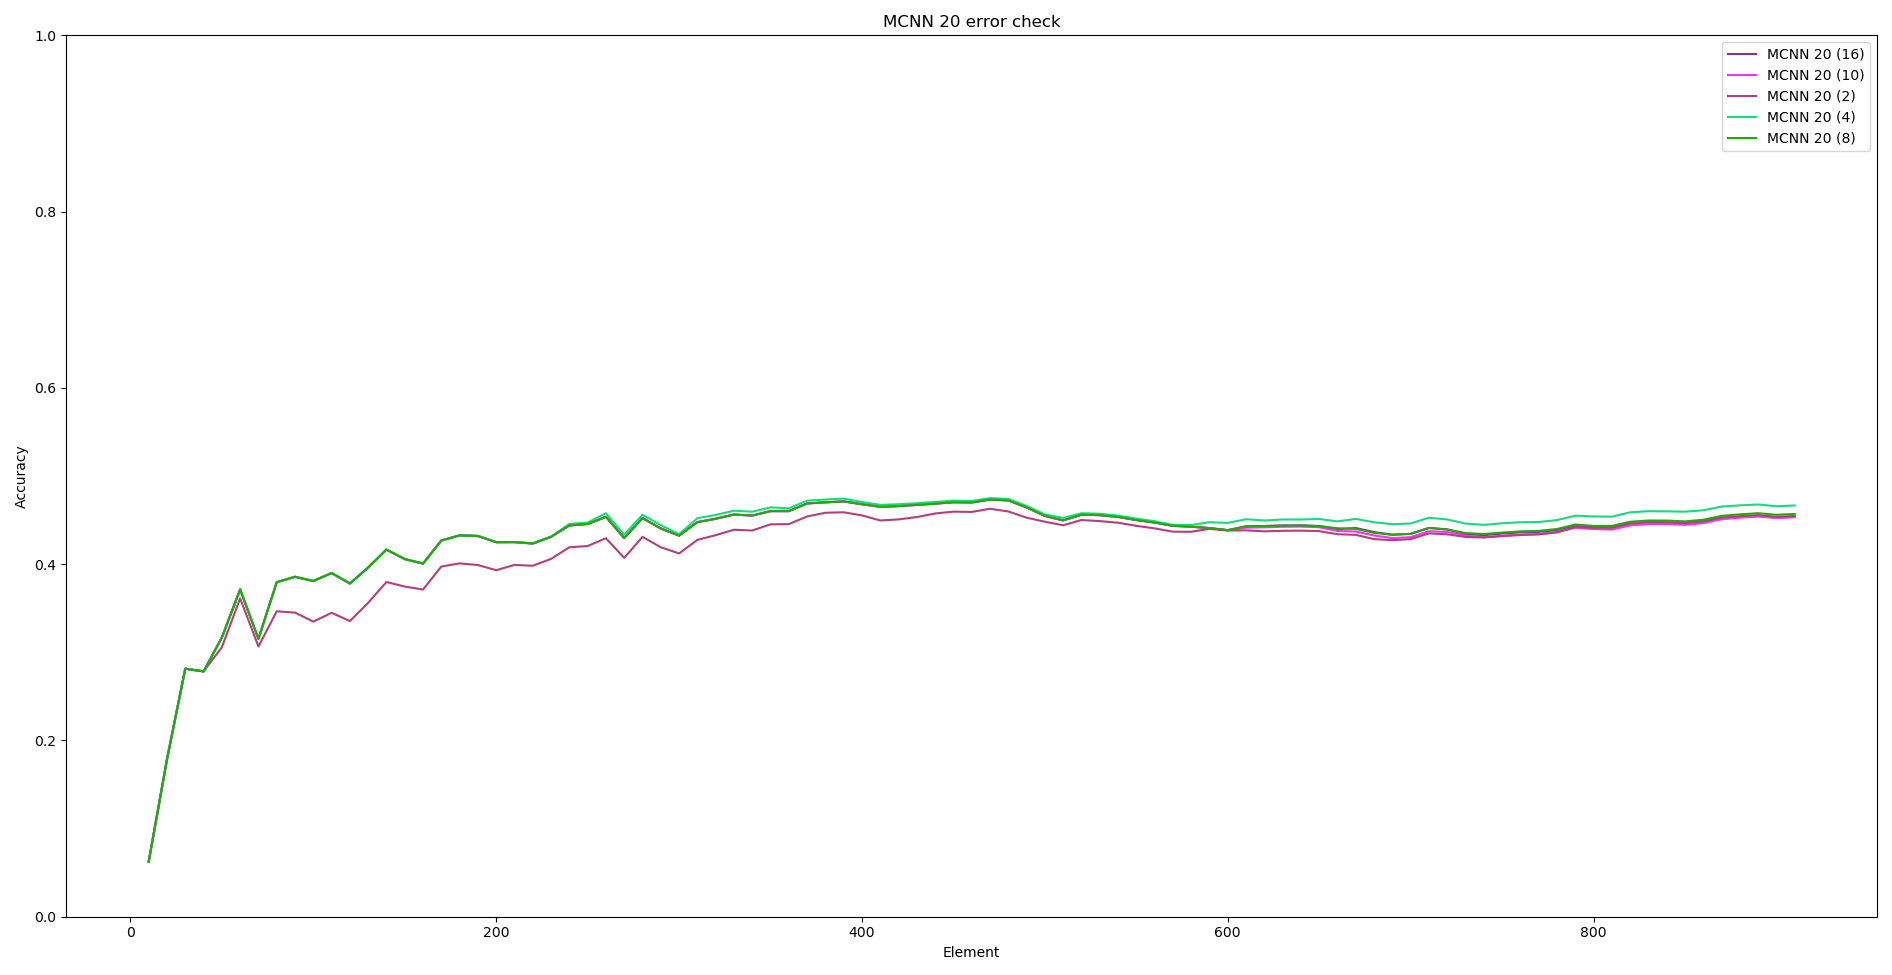
\includegraphics[width=\linewidth]{figures/Banos_S1_shuf_MCNN_20_error_check.png}
         \caption{20 clusters}
     \end{subfigure}
     \begin{subfigure}[b]{0.49\textwidth}
         \centering
		 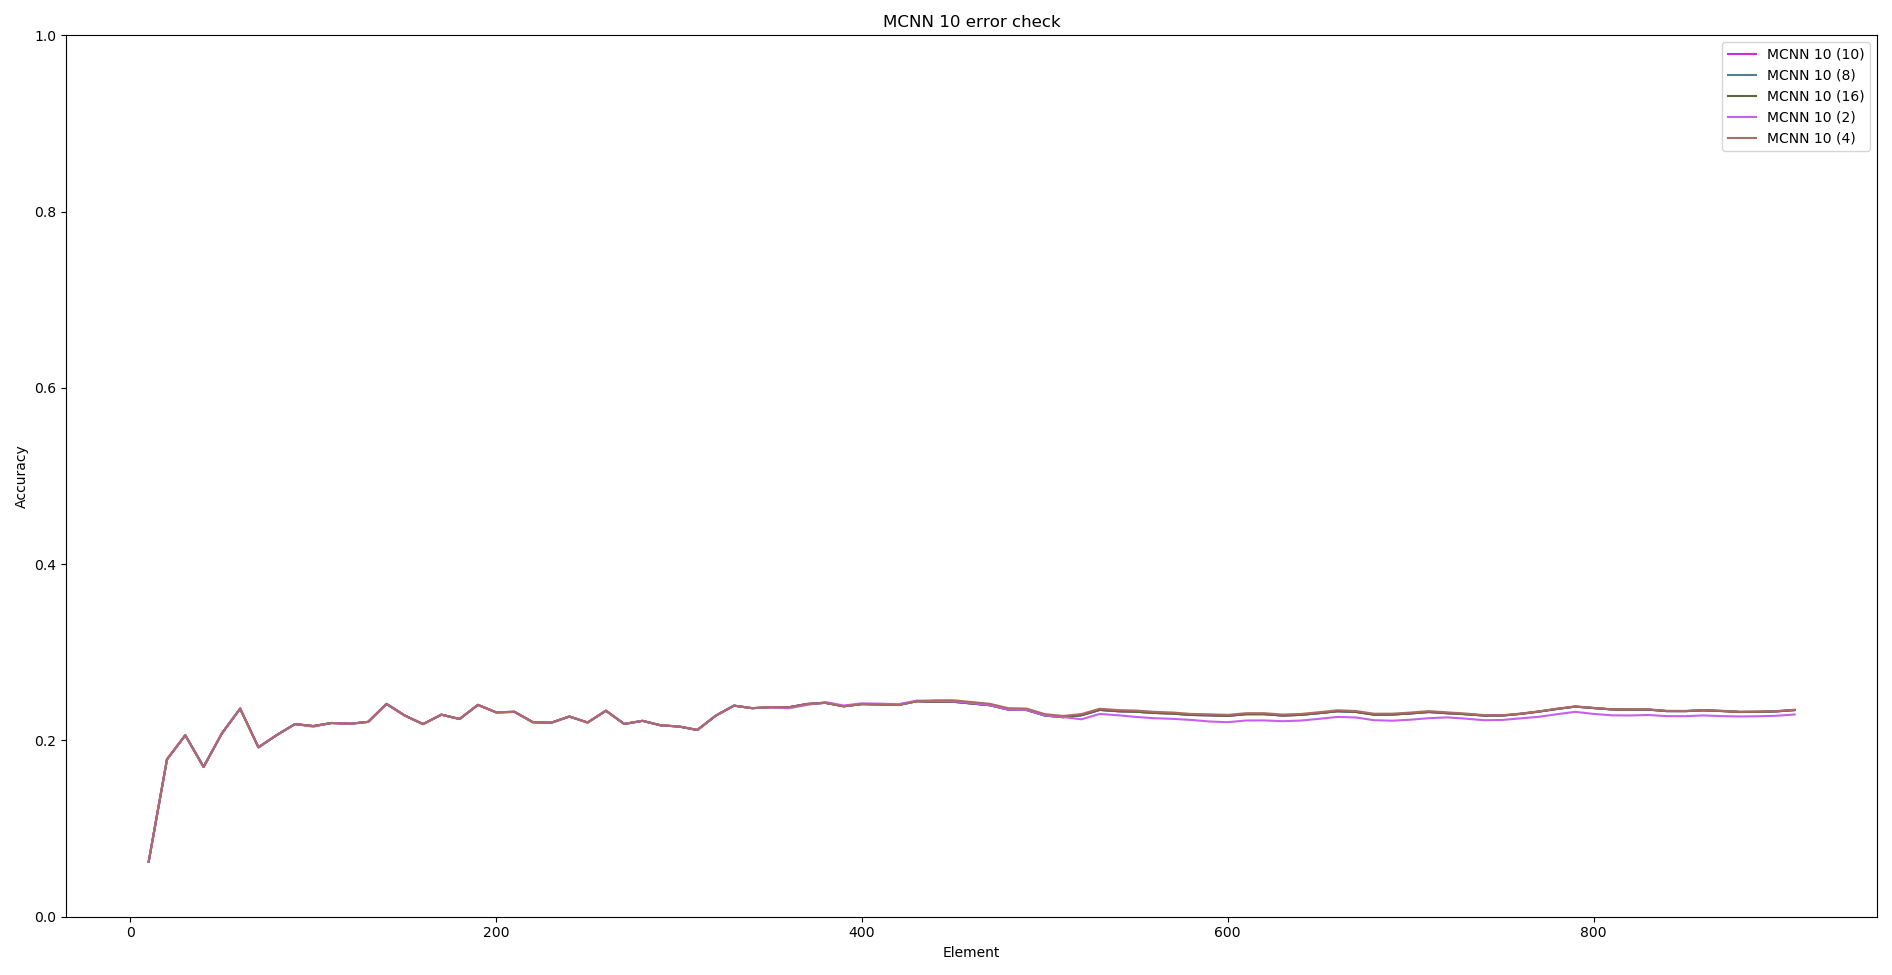
\includegraphics[width=\linewidth]{figures/Banos_S1_shuf_MCNN_10_error_check.png}
         \caption{10 clusters}
     \end{subfigure}
	\caption{MCNN error}
	\label{fig:mcnn-tuning-error}
\end{figure}

\subsection{Mondrian Tuning}
Figure~\ref{fig:mondrian-tuning} show the impact of the Mondrian parameters on
the accuracy. Occasionnaly, dashed lines are used to emphasis the minimum and
the maximum.
\begin{figure}
     \centering
     \begin{subfigure}[b]{0.49\textwidth}
         \centering
         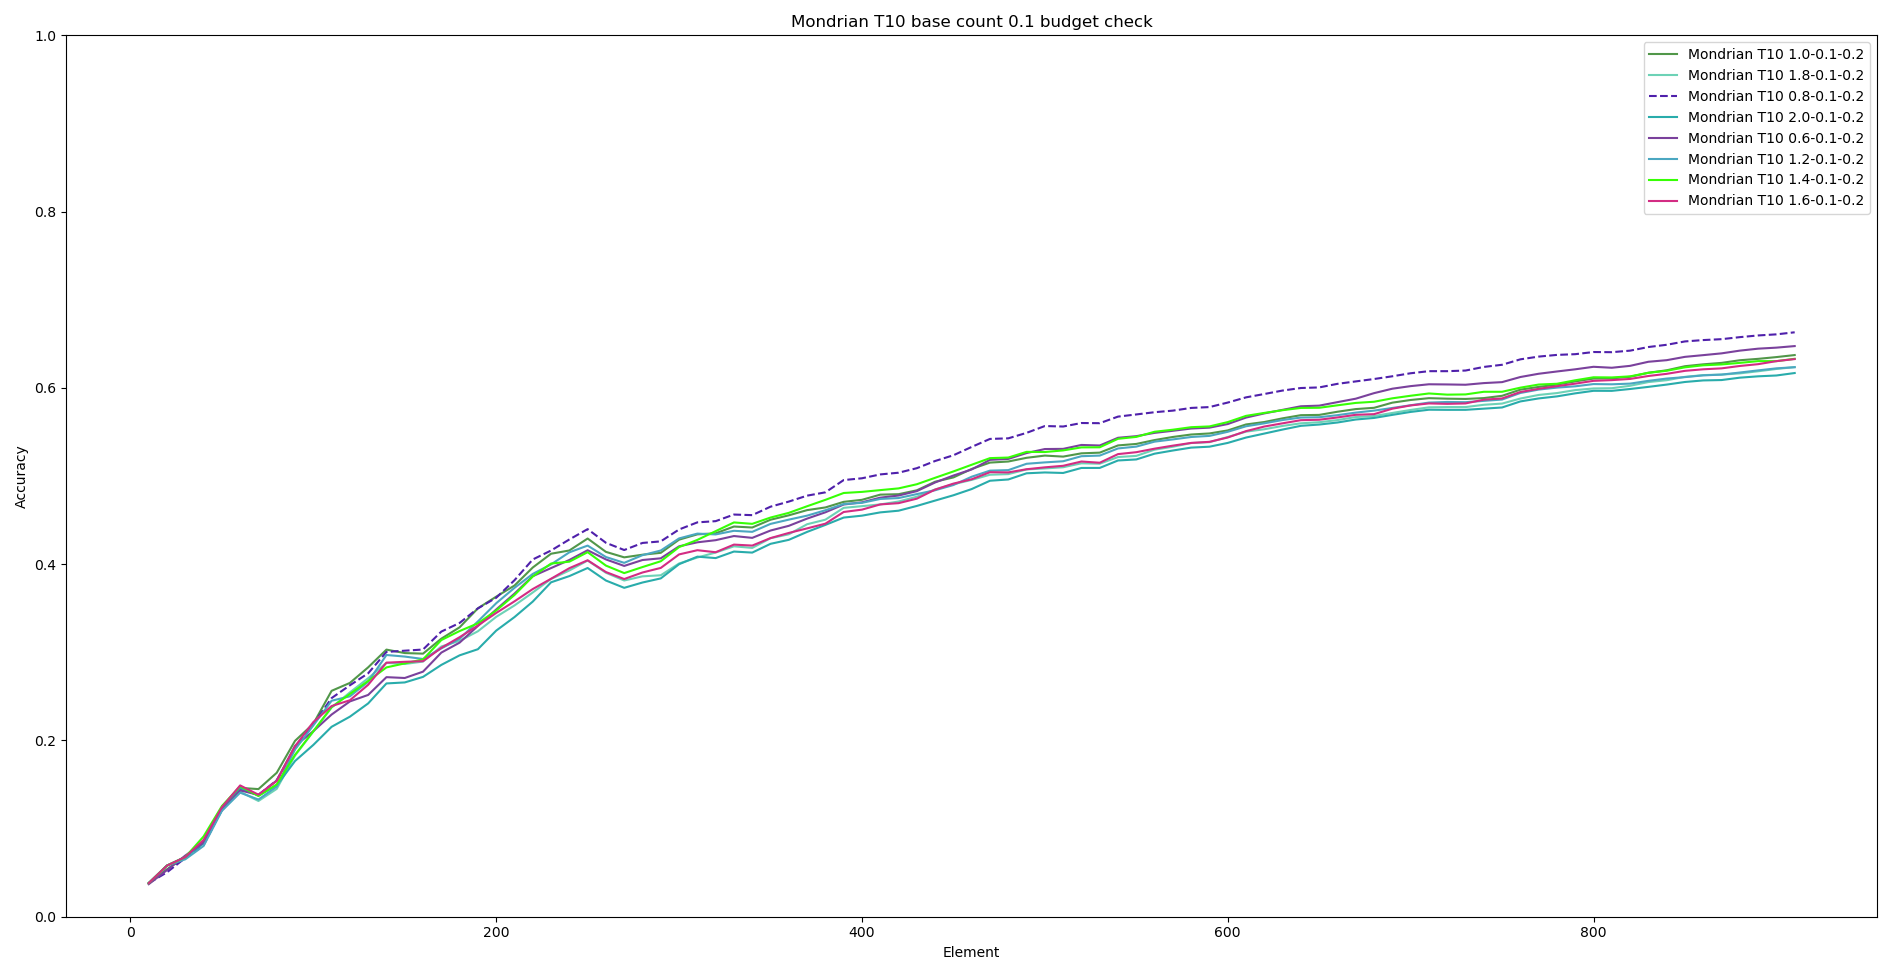
\includegraphics[width=\textwidth]{figures/Banos_S1_shuf_Mondrian_T10_bc_0.1_budget_check.png}
         \caption{Impact of the $budget$ with 10 trees, a base count of $0.1$, and discount factor of $0.2$.}
     \end{subfigure}
     \hfill
     \begin{subfigure}[b]{0.49\textwidth}
         \centering
         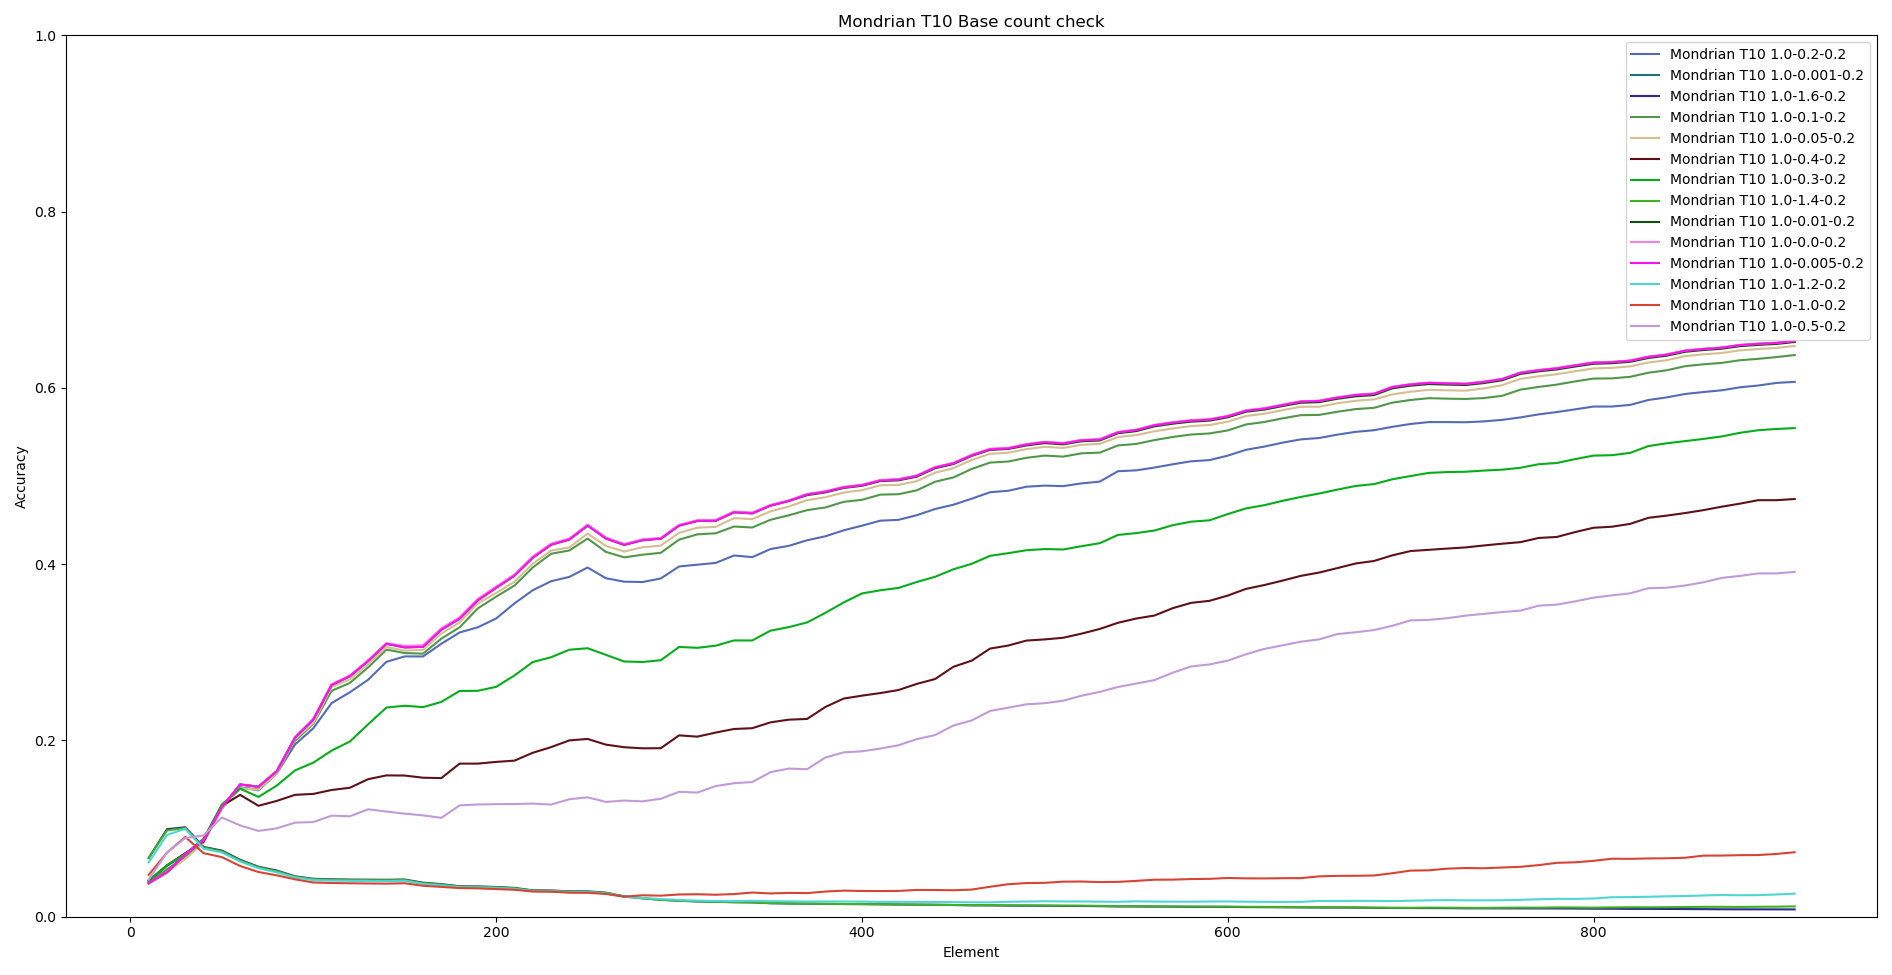
\includegraphics[width=\textwidth]{figures/Banos_S1_shuf_Mondrian_T10_check.png}
         \caption{Impact of the base count with 10 trees, a budget of $1.0$, and a discount factor of $0.2$.}
     \end{subfigure}
     \hfill
     \begin{subfigure}[b]{0.49\textwidth}
         \centering
         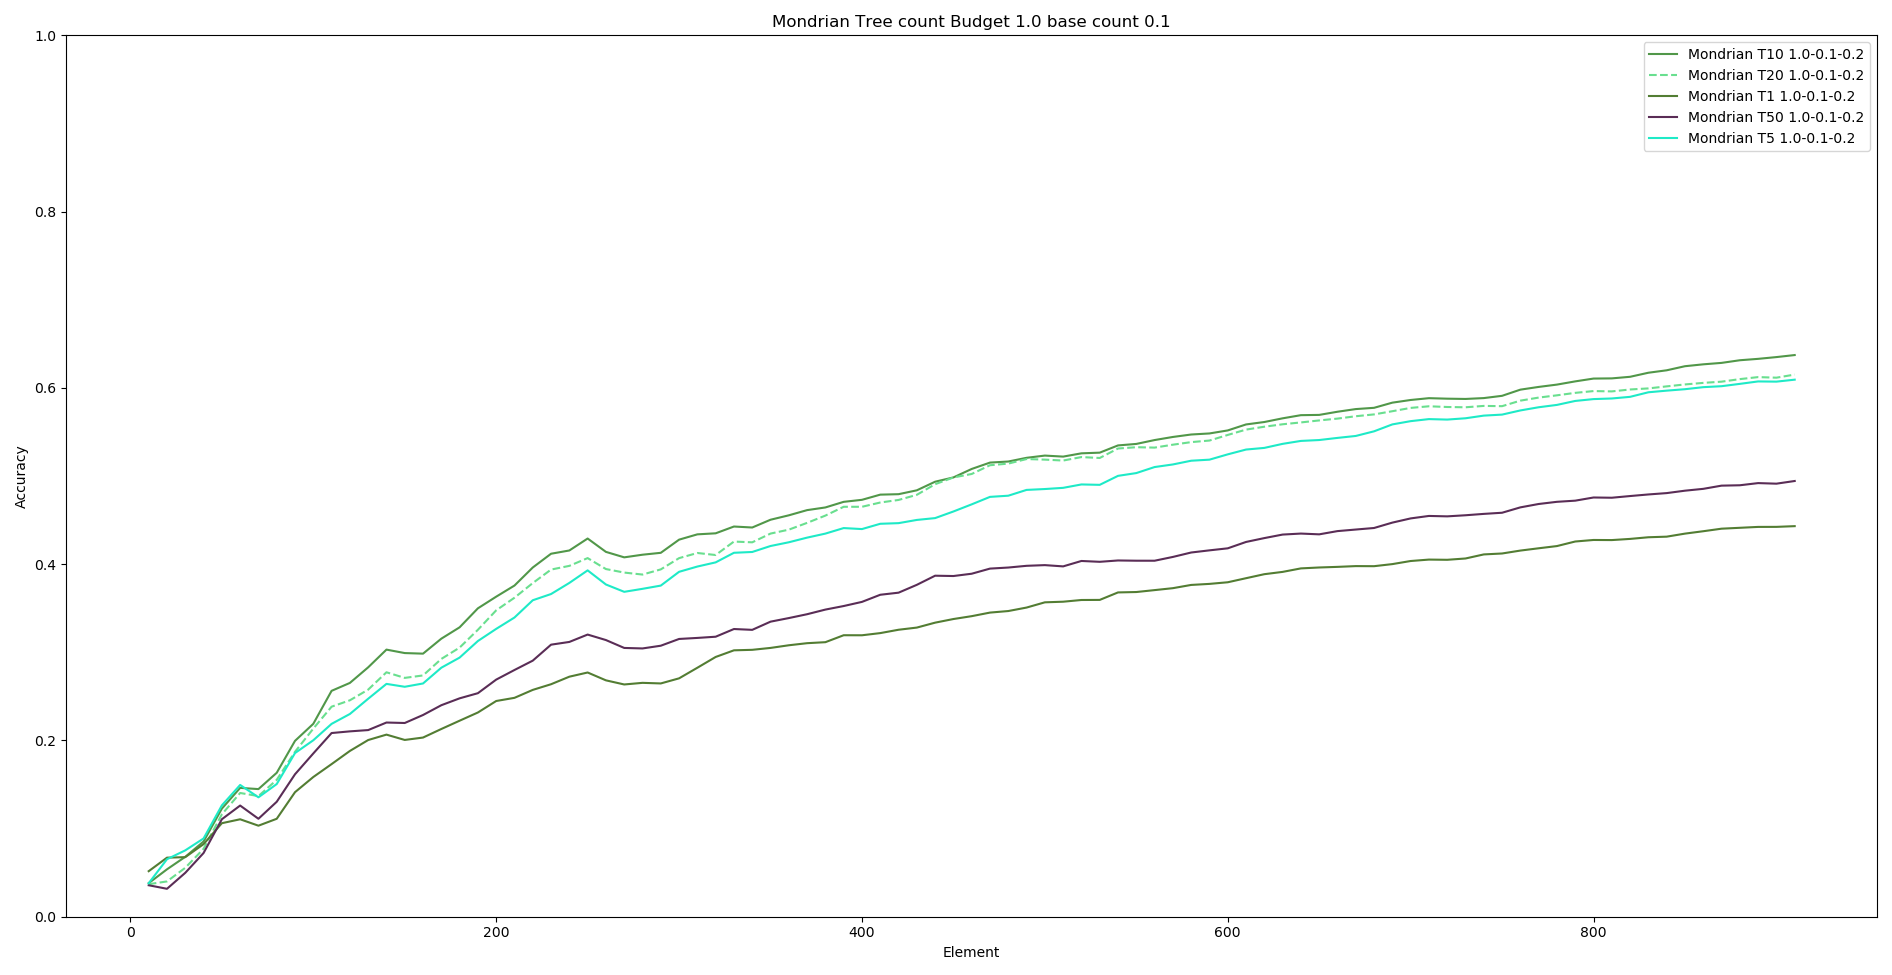
\includegraphics[width=\textwidth]{figures/Banos_S1_shuf_Mondrian_tree_count_fixed_other_bc0.1.png}
         \caption{Impact of the tree count with a budget of $1.0$, a base count of $0.1$, and a discount factor of $0.2$.}
     \end{subfigure}
     \begin{subfigure}[b]{0.49\textwidth}
         \centering
         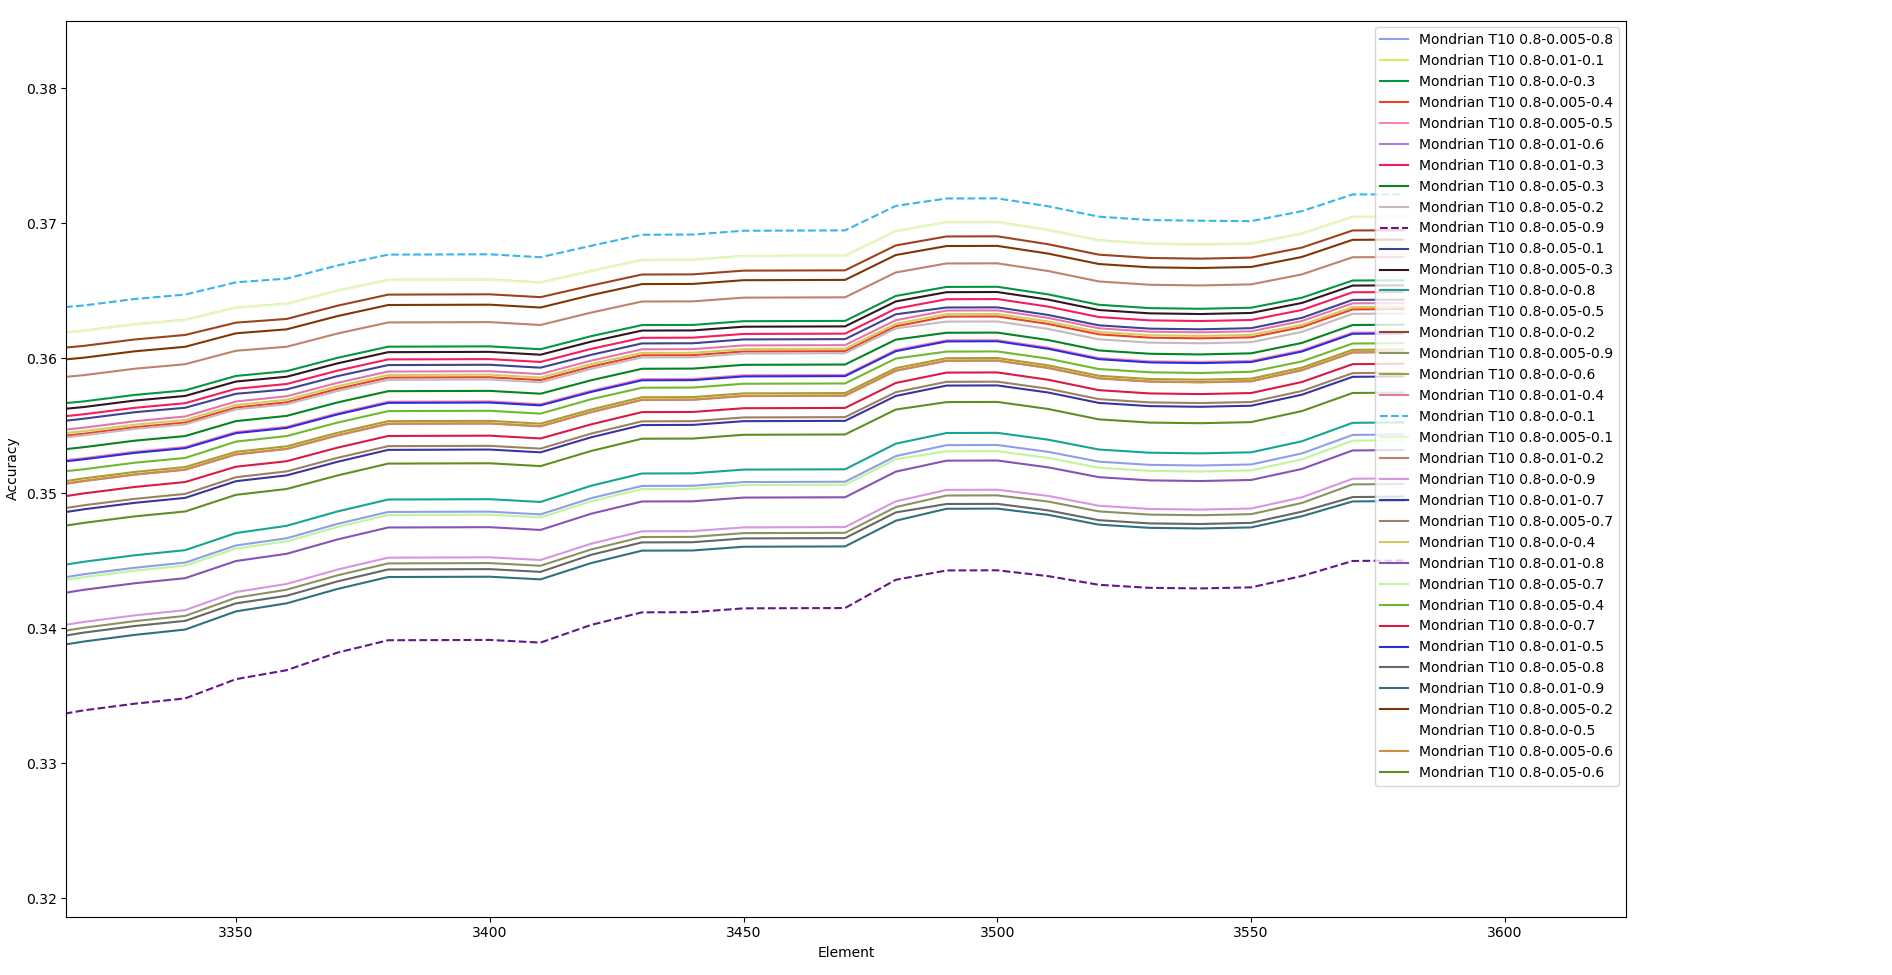
\includegraphics[width=\textwidth]{figures/Banos_S1_disount_check.png}
         \caption{Impact of the discount factor with 10 trees, a budget of $1.0$, and a base count of $0.1$.}
     \end{subfigure}
        \caption{Mondrian tuning results.}
        \label{fig:mondrian-tuning}
\end{figure}

